% !TeX encoding = UTF-8
% !TeX program = xelatex
% !TeX spellcheck = en_US

\documentclass[degree=bachelor]{thuthesis}
  % 学位 degree:
  %   doctor | master | bachelor | postdoc
  % 学位类型 degree-type:
  %   academic(默认)| professional
  % 语言 language
  %   chinese(默认)| english
  % 字体库 fontset
  %   windows | mac | fandol | ubuntu
  % 研究生院建议终版使用 Windows 平台的字体编译


% 论文基本配置,加载宏包等全局配置
% !TeX root = ./thuthesis-example.tex

% 论文基本信息配置

\thusetup{
  %******************************
  % 注意:
  %   1. 配置里面不要出现空行
  %   2. 不需要的配置信息可以删除
  %   3. 建议先阅读文档中所有关于选项的说明
  %******************************
  %
  % 输出格式
  %   选择打印版(print)或用于提交的电子版(electronic),前者会插入空白页以便直接双面打印
  %
  output = print,
  %
  % 标题
  %   可使用“\\”命令手动控制换行
  %
  title  = {基于安全属性检查的程序上界验证方法},
  title* = {A safety-check based approach of program bound validation},
  %
  % 学位
  %   1. 学术型
  %      - 中文
  %        需注明所属的学科门类,例如:
  %        哲学、经济学、法学、教育学、文学、历史学、理学、工学、农学、医学、
  %        军事学、管理学、艺术学
  %      - 英文
  %        博士:Doctor of Philosophy
  %        硕士:
  %          哲学、文学、历史学、法学、教育学、艺术学门类,公共管理学科
  %          填写“Master of Arts“,其它填写“Master of Science”
  %   2. 专业型
  %      直接填写专业学位的名称,例如:
  %      教育博士、工程硕士等
  %      Doctor of Education, Master of Engineering
  %   3. 本科生不需要填写
  %
  degree-name  = {工学学士},
  degree-name* = {Bachelor of Science},
  %
  % 培养单位
  %   填写所属院系的全名
  %
  department = {计算机科学与技术系},
  %
  % 学科
  %   1. 学术型学位
  %      获得一级学科授权的学科填写一级学科名称,其他填写二级学科名称
  %   2. 工程硕士
  %      工程领域名称
  %   3. 其他专业型学位
  %      不填写此项
  %   4. 本科生填写专业名称,第二学位论文需标注“(第二学位)”
  %
  discipline  = {计算机科学与技术},
  discipline* = {Computer Science and Technology},
  %
  % 姓名
  %
  author  = {},
  author* = {},
  %
  % 指导教师
  %   中文姓名和职称之间以英文逗号“,”分开,下同
  %
  supervisor  = {},
  supervisor* = {},
  %
  % 副指导教师
  %
  %associate-supervisor  = {陈文光, 教授},
  %associate-supervisor* = {Professor Chen Wenguang},
  %
  % 联合指导教师
  %
  % co-supervisor  = {某某某, 教授},
  % co-supervisor* = {Professor Mou Moumou},
  %
  % 日期
  %   使用 ISO 格式;默认为当前时间
  %
  % date = {2019-07-07},
  %
  % 是否在中文封面后的空白页生成书脊(默认 false)
  %
  include-spine = false,
  %
  % 密级和年限
  %   秘密, 机密, 绝密
  %
  % secret-level = {秘密},
  % secret-year  = {10},
  %
  % 博士后专有部分
  %
  % clc                = {分类号},
  % udc                = {UDC},
  % id                 = {编号},
  % discipline-level-1 = {计算机科学与技术},  % 流动站(一级学科)名称
  % discipline-level-2 = {系统结构},          % 专业(二级学科)名称
  % start-date         = {2011-07-01},        % 研究工作起始时间
}

% 载入所需的宏包

% 定理类环境宏包
\usepackage{amsthm}
% 也可以使用 ntheorem
% \usepackage[amsmath,thmmarks,hyperref]{ntheorem}

\thusetup{
  %
  % 数学字体
  % math-style = GB,  % GB | ISO | TeX
  math-font  = xits,  % sitx | xits | libertinus
}

% 可以使用 nomencl 生成符号和缩略语说明
% \usepackage{nomencl}
% \makenomenclature

% 表格加脚注
\usepackage{threeparttable}

% 表格中支持跨行
\usepackage{multirow}

% 固定宽度的表格。
% \usepackage{tabularx}

% 跨页表格
\usepackage{longtable}

% 算法
\usepackage{algorithm}
\usepackage{algorithmic}

% 量和单位
\usepackage{siunitx}

\usepackage{rotating}

% 参考文献使用 BibTeX + natbib 宏包
% 顺序编码制
\usepackage[sort]{natbib}
\bibliographystyle{thuthesis-numeric}

% 著者-出版年制
% \usepackage{natbib}
% \bibliographystyle{thuthesis-author-year}

% 本科生参考文献的著录格式
% \usepackage[sort]{natbib}
% \bibliographystyle{thuthesis-bachelor}

% 参考文献使用 BibLaTeX 宏包
% \usepackage[backend=biber,style=thuthesis-numeric]{biblatex}
% \usepackage[backend=biber,style=thuthesis-author-year]{biblatex}
% \usepackage[backend=biber,style=apa]{biblatex}
% \usepackage[backend=biber,style=mla-new]{biblatex}
% 声明 BibLaTeX 的数据库
% \addbibresource{ref/refs.bib}

\usepackage{tikz}
\usetikzlibrary{automata, positioning, arrows, shapes}
\tikzset{
    ->, % makes the edges directed
    >=stealth, % makes the arrow heads bold
    node distance=3cm, % specifies the minimum distance between two nodes. Change if necessary.
    every state/.style={thick, fill=gray!10}, % sets the properties for each ’state’ node
    initial text=$ $, % sets the text that appears on the start arrow
}
\usepackage{minted}
% 定义所有的图片文件在 figures 子目录下
\graphicspath{{figures/}}

% 数学命令
\makeatletter
\newcommand\dif{%  % 微分符号
  \mathop{}\!%
  \ifthu@math@style@TeX
    d%
  \else
    \mathrm{d}%
  \fi
}
\makeatother

% hyperref 宏包在最后调用
\usepackage{hyperref}



\begin{document}

% 封面
\maketitle

% 学位论文指导小组、公开评阅人和答辩委员会名单
%% !TeX root = ../main.tex

\begin{committee}[name={学位论文指导小组、公开评阅人和答辩委员会名单}]

  \newcolumntype{C}[1]{@{}>{\centering\arraybackslash}p{#1}}

  \section*{指导小组名单}

  \begin{center}
    \begin{tabular}{C{3cm}C{3cm}C{9cm}@{}}
      李XX & 教授     & 清华大学 \\
      王XX & 副教授   & 清华大学 \\
      张XX & 助理教授 & 清华大学 \\
    \end{tabular}
  \end{center}


  \section*{公开评阅人名单}

  \begin{center}
    \begin{tabular}{C{3cm}C{3cm}C{9cm}@{}}
      刘XX & 教授   & 清华大学                    \\
      陈XX & 副教授 & XXXX大学                    \\
      杨XX & 研究员 & 中国XXXX科学院XXXXXXX研究所 \\
    \end{tabular}
  \end{center}


  \section*{答辩委员会名单}

  \begin{center}
    \begin{tabular}{C{2.75cm}C{2.98cm}C{4.63cm}C{4.63cm}@{}}
      主席 & 赵XX                  & 教授                    & 清华大学       \\
      委员 & 刘XX                  & 教授                    & 清华大学       \\
          & \multirow{2}{*}{杨XX} & \multirow{2}{*}{研究员} & 中国XXXX科学院 \\
          &                       &                         & XXXXXXX研究所  \\
          & 黄XX                  & 教授                    & XXXX大学       \\
          & 周XX                  & 副教授                  & XXXX大学       \\
      秘书 & 吴XX                  & 助理研究员              & 清华大学       \\
    \end{tabular}
  \end{center}

\end{committee}



% 也可以导入 Word 版转的 PDF 文件
% \begin{committee}[file=figures/committee.pdf]
% \end{committee}


% 使用授权的说明
%\copyrightpage
% 将签字扫描后授权文件 scan-copyright.pdf 替换原始页面
% \copyrightpage[file=copyright.pdf]

\frontmatter
% !TeX root = ../main.tex

% 中英文摘要和关键字

\begin{abstract}

    对程序复杂度和执行上界的分析由来已久。随着验证和综合技术的发展,自动化上界生成成为受到关注的研究方向。但是,现有工具所生成的上界的正确性并没有得到验证,实际中更是出现了生成上界为错误的情况。如何验证上界表达式的正确性是本文研究的主要问题。
    
    安全属性是形式验证特别关注的一类属性规范,描述了系统不会产生规定之外的行为。安全属性的检查已有长足的发展,近年在软件模型检测领域得到了广泛的应用。本文进行上界验证的基本思路是通过程序变换,将问题归约为安全属性的检查,从而利用现有的验证技术完成正确性的证明。
    
    本文在\texttt{Ultimate}框架内实现了验证算法。实验分析表明,本文方法能有效地验证程序的上界。

  % 关键词用“英文逗号”分隔,输出时会自动处理为正确的分隔符
  \thusetup{
    keywords = {上界验证, 安全属性检查, 形式化验证, 程序分析, 自动化验证},
  }
\end{abstract}

\begin{abstract*}
  Analyzing the complexity and execution bound of program has a long tradition. With the development of verification and synthesis technologies, automated bound analysis has become an interesting research field. However, the bound generated by existing analysis tools is not validated, which entails the possibility of erroneous bound. How to verify a bound expression is the main issue addressed in this paper.
  
  Of special interests in formal verification are safety properties, which assert the system never engenders any prohibited behavior. Safety properties checking has been massively studied and in recent years it has been used in software model checking. The methodology in the paper is to reduce bound verification to safety property checking via program instrumentation and utilize existing verification technologies.
  
  We implemented the bound verification algorithm in the \texttt{Ultimate} framework. Experimental analysis shows that our method can effectively verify program bound.

  % Use comma as seperator when inputting
  \thusetup{
    keywords* = {bound verification, safety property check, formal verification, program analysis, automated verification},
  }
\end{abstract*}


% 目录
\tableofcontents

% 符号对照表
% !TeX root = ../main.tex

\begin{denotation}[3cm]
  \item[CFG] 控制流图
  \item[WCET] 最坏情况执行时间
  \item[WCCC] 最坏情况计算复杂度
  \item[\textbf{Imp}] 论文形式化定义的一种简单命令式语言
  \item[SSA] 静态单赋值形式
  \item[$l_{err}$] 错误位置
  \item[$L_{h}$] 自然循环
  \item[$l_{h}$] 循环头
  \item[$\pi$] 程序中的一条路径
  \item[$\tau$] 程序的变迁关系
\end{denotation}


% 也可以使用 nomencl 宏包,需要在导言区
% \usepackage{nomencl}
% \makenomenclature

% 在这里输出符号说明
% \printnomenclature[3cm]

% 在正文中的任意为都可以标题
% \nomenclature{PI}{聚酰亚胺}
% \nomenclature{MPI}{聚酰亚胺模型化合物,N-苯基邻苯酰亚胺}
% \nomenclature{PBI}{聚苯并咪唑}
% \nomenclature{MPBI}{聚苯并咪唑模型化合物,N-苯基苯并咪唑}
% \nomenclature{PY}{聚吡咙}
% \nomenclature{PMDA-BDA}{均苯四酸二酐与联苯四胺合成的聚吡咙薄膜}
% \nomenclature{MPY}{聚吡咙模型化合物}
% \nomenclature{As-PPT}{聚苯基不对称三嗪}
% \nomenclature{MAsPPT}{聚苯基不对称三嗪单模型化合物,3,5,6-三苯基-1,2,4-三嗪}
% \nomenclature{DMAsPPT}{聚苯基不对称三嗪双模型化合物(水解实验模型化合物)}
% \nomenclature{S-PPT}{聚苯基对称三嗪}
% \nomenclature{MSPPT}{聚苯基对称三嗪模型化合物,2,4,6-三苯基-1,3,5-三嗪}
% \nomenclature{PPQ}{聚苯基喹噁啉}
% \nomenclature{MPPQ}{聚苯基喹噁啉模型化合物,3,4-二苯基苯并二嗪}
% \nomenclature{HMPI}{聚酰亚胺模型化合物的质子化产物}
% \nomenclature{HMPY}{聚吡咙模型化合物的质子化产物}
% \nomenclature{HMPBI}{聚苯并咪唑模型化合物的质子化产物}
% \nomenclature{HMAsPPT}{聚苯基不对称三嗪模型化合物的质子化产物}
% \nomenclature{HMSPPT}{聚苯基对称三嗪模型化合物的质子化产物}
% \nomenclature{HMPPQ}{聚苯基喹噁啉模型化合物的质子化产物}
% \nomenclature{PDT}{热分解温度}
% \nomenclature{HPLC}{高效液相色谱(High Performance Liquid Chromatography)}
% \nomenclature{HPCE}{高效毛细管电泳色谱(High Performance Capillary lectrophoresis)}
% \nomenclature{LC-MS}{液相色谱-质谱联用(Liquid chromatography-Mass Spectrum)}
% \nomenclature{TIC}{总离子浓度(Total Ion Content)}
% \nomenclature{\textit{ab initio}}{基于第一原理的量子化学计算方法,常称从头算法}
% \nomenclature{DFT}{密度泛函理论(Density Functional Theory)}
% \nomenclature{$E_a$}{化学反应的活化能(Activation Energy)}
% \nomenclature{ZPE}{零点振动能(Zero Vibration Energy)}
% \nomenclature{PES}{势能面(Potential Energy Surface)}
% \nomenclature{TS}{过渡态(Transition State)}
% \nomenclature{TST}{过渡态理论(Transition State Theory)}
% \nomenclature{$\increment G^\neq$}{活化自由能(Activation Free Energy)}
% \nomenclature{$\kappa$}{传输系数(Transmission Coefficient)}
% \nomenclature{IRC}{内禀反应坐标(Intrinsic Reaction Coordinates)}
% \nomenclature{$\nu_i$}{虚频(Imaginary Frequency)}
% \nomenclature{ONIOM}{分层算法(Our own N-layered Integrated molecular Orbital and molecular Mechanics)}
% \nomenclature{SCF}{自洽场(Self-Consistent Field)}
% \nomenclature{SCRF}{自洽反应场(Self-Consistent Reaction Field)}



% 正文部分
\mainmatter
\newcommand{\assign}{:=}
\newcommand{\colons}{\,:\,}
\newcommand{\nin}{\not\in}
\newcommand{\textdots}{...}
\newcommand{\tmmathbf}[2]{\ensuremath{\boldsymbol{#1}}}
\newcommand{\tmop}[1]{\ensuremath{\operatorname{#1}}}
\newcommand{\tmtextbf}[1]{{\bfseries{#1}}}
\newcommand\todo[1]{\textcolor{red}{#1}}
\newcommand{\loopus}{\texttt{Loopus}}
\newcommand{\ultimate}{\texttt{Ultimate}}
% !TeX root = ../main.tex

\chapter{引言}

\section{研究背景}

自从通用计算模型\cite{turing_computable_1937}被提出以来,随着计算机科学和信息技术的发展,计算机程序已在各领域被广泛应用,逐渐成为社会生活中不可或缺的组成部分。人们通过形式语言来设计算法,描述计算机要执行的工作,但是模型缺陷或编码错误往往会引入造成严重后果的错误。研究程序正确性的验证方法因此具有重要意义。

\subsection{资源分析与上界分析}
\label{section:chap1-bound-analysis-intro}
程序的正确性是由一系列预期属性或规范所规定的。程序分析技术的目标即是通过对程序进行综合考察,分析程序的各类动态属性。资源分析(cost/resource analysis)是程序分析的一个研究方向,它假设程序有着一定的资源消耗模型(consumption model),期望通过对程序结构和语义的分析,预先得出或近似程序资源消耗量。

资源分析的一个主要应用场景是在嵌入式系统的分析中,得出实时控制系统的最坏情况执行时间\cite{wilhelm_worst-case_2008}(worst case execution time,简称WCET),此时,程序的执行时间被视为其消耗的“资源”;另外一个应用场景是分析安全攸关软件的信息安全级别,此时,系统中机密信息的泄漏程度被作为程序消耗的“资源”进行分析\cite{smith_foundations_2009}。

上界分析(bound analysis\footnote{直译为界分析,但实际场景中一般只会关注上界的存在})类似于对程序时间复杂度所做的资源分析,不过,上界分析一般采取更为抽象和高层次的复杂度表示。程序的执行时间,如上述的WCET指标,受到硬件实现细节的诸多影响,不利于理论的分析。现有的上界分析工具能从不同的粒度对上界进行分析,比如,从程序底层的变迁系统表示出发分析状态转移的次数,或者从程序控制流层面出发分析循环的迭代次数\cite{sinn_simple_2014},以及从函数间调用的层面分析递归的实例数目\cite{gulwani_speed_2009, gulwani_control-flow_2009}等。

\subsection{研究动机}

自动上界生成工具是以完全自动化的方式寻找输入程序的界。它们采取了不同的策略和技术,包括抽象解释技术、软件模型检测技术及计算代数理论等。其中,由奥地利维也纳技术大学的学者开发的\texttt{Loopus} 工具 \cite{sinn_simple_2014,zuleger_bound_2011,sinn_difference_2015,sinn_complexity_2017}是近期较为出色的工具。我们考察了其于2014年在测试集上进行的测验\footnote{原始测试结果见\url{https://forsyte.at/static/people/sinn/loopus/CAV14/comparisonLoopusKoATPUBSRank.html}},结果发现其计算得到的上界表达式出现了错误。比如,对于代码\ref{listing:chap1-motivating-program}中的C语言程序,\texttt{Loopus}给出的循环上界是$b - 1 + b \times (b - 1)$。

\begin{listing}

\begin{minted}
[
frame=lines,
framesep=2mm,
baselinestretch=1,
fontsize=\footnotesize,
linenos
]{c}
void ex02(int a, int b, int c) {
  a = 0;
  while (b >= 1 + a) {
      c = 0;
      while (1) {
        if (a >= c) {
          c = c + 1;
        }
        else if (c >= a + 1) {
          a = a + 1;
          break;
        }
        else if (1) {
          c = 1;
          a = 1;
          b = 1;
          break;
        }
        else
          return;
      }
  }
  return;
}
\end{minted}

\caption{一个\texttt{Loopus}所给出上界为错误的C语言程序}
\label{listing:chap1-motivating-program}
\end{listing}

循环上界将在下文形式化地定义,简单来说,其类似于程序中循环的迭代次数。显然,$b - 1 + b \times (b - 1)$并不是上述程序的上界,只需考虑当$b=1$时的情况\footnote{a和c的初始值不影响循环的迭代次数}:此时循环共迭代3次(内层循环2次,外层循环1次),多于带入表达式中所计算出的0次。

自动验证工具由于设计复杂,实现的难度较高,有可能出现编码问题,影响工具的可靠性,而确保验证工具的可靠性是至关重要的。比如,上例表明了在上界分析领域进行结果验证的必要性。对于自动上界生成工具所给出的结果,即上界表达式,需要一种方法检查其是否确为程序的上界,这对于增强系统的可靠性和置信度很有价值。本文即研究如何对程序的上界进行验证。

目前,没有专门进行上界验证的工作。有关自动上界生成领域的进展,参看附录\ref{cha:survey}的文献综述报告。

\section{本论文的结构}

本文的剩余部分安排如下:

第二章是前置定义,包含和上界验证相关的若干概念的形式化定义,包括程序的语法和语义、控制流图表示、自然循环、循环上界和安全属性检查等四个部分,此外还简要介绍了安全属性检查的原理。为力求完整和精确,这一章的形式化较多。

第三章提出基于安全属性检查的上界验证算法。首先关注的是单一循环的验证,分为全局上界和局部上界两个部分,并分别给出了问题归约方法的细节以及这一归约的正确性证明;其次通过“证明结构”这一概念,支持对多循环程序的验证。

第四章是算法实现和实验评估。本章首先概述了实现所基于的Ultimate框架及所用到的两种验证专用语言,其次介绍实现的细节。最后,给出了实验测试集的选择和筛选方法,以及工具在其上的实验结果。

第五章是结论和展望,对于目前工作进行了总结,对进一步工作的可能方向进行了讨论。


% !TeX root = ../main.tex

\chapter{前置定义}

程序的上界(upper bound)是一种抽象的模型,目的是对程序在真实环境下的实际执行时间和效率进行近似。正如在第\ref{section:chap1-bound-analysis-intro}节中指出的那样,最坏情况执行时间(WCET)这一指标受到诸多因素的影响,难以事先确定并进行分析。为此,需要一种在形式上准确可行的方法,以便于较为准确地预测从而改进程序的性能。

在计算理论中,通常使用图灵机执行的最大长度或者移动的最大距离等作为这种抽象的模型。这是一种可行但过于底层的做法,实际的程序中有着各式复杂的结构,需要更加高层次的表示。

本篇论文为避免涉及实际编程语言的诸多细节,简化表示和方便陈述,构建了一个简单的命令式语言\tmtextbf{Imp}。其特点是单例程,变量都为整型,且只含有简单表达式\footnote{指表达式在求值时无副作用(side-effects)}。此章下文将详细地对其进行描述,并给出程序、循环、上界等概念的形式化定义。下一章节将在此基础上给出主要的算法。第四章将描述如何将其应用在C语言程序的验证之中。

\section{表达式与语句}

这一节定义了工作语言\tmtextbf{Imp}的若干构件的语法和语义。首先给出表达式的语法的定义:

\begin{definition}
  $Var$是一组程序变量的集合,其中$x \in \tmop{Var}$代表整型变量。
\end{definition}

\begin{definition}
  \label{def:chap2-arith-expr}
  
  A是由变量和整型常量构成的算数表达式的集合。算数表达式由下列规则定义:
  
  \[ 
  a := x \mid i \mid a \mathbin{\mathbf{op}} a \mid - a 
  \]
     
  其中$x \in \tmop{Var}, i \in \mathbb{Z},  \mathbf{op} \in \{ +, -, \times, / \}$,其语义为标准语义。
\end{definition}

\begin{definition}
  设$\bot$代表假值,$\top$代表真值。B是由变量和整型常量构成的布尔表达式的集合。布尔表达式由下列规则定义:
  \[ b := a \mathbin{\mathbf{cop}} a \mid b \mathbin{\mathbf{bop}} b
     \mid \neg b \mid \bot \mid \top \]
  其中$a \in A, \mathbf{cop} \in \{ >, <, \geqslant, \leqslant,
  =, \neq \}, \mathbf{bop} \in \{ \wedge, \vee, \rightarrow
  \}$,其语义为标准语义。
\end{definition}

表达式的求值是在一定的状态中进行的,状态(memory state)代表了在程序执行的某个瞬间,程序中各变量的值:

\begin{definition}
  程序的状态是一个将变量映射为整型值的函数,即$s \in \tmop{Var} \rightarrow \mathbb{Z}$。S是状态的集合。将状态s在变量x上的值更新为$a \in \mathbb{Z}$,记为$s [x / a]$,定义如下:
  
  \[ s [x / a] (y) = \left\{ \begin{array}{cc}
       s (y) & x \neq y\\
       a & x = y
     \end{array} \right. \]
     
\end{definition}

给定表达式和当前状态,可以递归地计算出表达式在当前状态下的值:

\begin{definition}
  算数表达式$a \in A$在状态s中的值是$\mathbb{Z}$中的元素,写作s(a),由下列规则定义:
  
  \[ s (a) = \left\{ \begin{array}{ll}
       s (x) & a = x\\
       i & a = i\\
       s (a_1)  \mathbin{\mathbf{op}} s (a_2) & a = a_1  \mathbin{\mathbf{op}} a_2\\
       - s (a_1) & a = - a_1
     \end{array} \right. \]
\end{definition}

\begin{definition}
  布尔表达式$b \in B$在状态s中的值是$\{ \bot, \top
  \}$中的元素,写作s(b),由下列规则定义:
  \[ s (b) = \left\{ \begin{array}{ll}
       s (a_1)  \mathbin{\mathbf{cop}} s (a_2) & b = a_1  \mathbin{\mathbf{cop}} a_2\\
       s (b_1)  \mathbin{\mathbf{bop}} s (b_2) & b = b_1  \mathbin{\mathbf{bop}} b_2\\
       \neg s (b_1)  & b = \neg b_1\\
       b & b = \bot \, \mathrm{or} \, \top
     \end{array} \right. \]
\end{definition}

命令式程序由一条条的语句(statement)组成,语句是对程序状态进行改变的操作,不同的语句具有不同的效果。我们考虑如下的语句集合:

\begin{definition}
  语句集Stmt是全体语句stmt的集合。语句由下列规则定义:
  \[ \tmop{stmt} := \mathbf{\tmop{skip}} \mid x = a \mid
     \mathbf{havoc} \, x \, \mid \mathbf{assume} \,b \, \mid
     \tmop{stmt} \mathbf{;} \tmop{stmt} \]
  其中,$x \in \tmop{Var}, a \in A, b \in B$。这五种语句也非形式化地称为空语句、赋值语句、非确定型赋值语句、假设断言语句和语句复合。
\end{definition}

\begin{definition}
  \label{def:chap2-semantics}
  语句stmt可视为状态集S上的一个关系,对任意两个状态$s_1$和$s_2$,用$\{ s_1 \} \tmop{stmt} \{ s_2 \}$表示$(s_1, s_2) \in \tmop{stmt}$。此关系可由如下的推导规则(inference rule)\footnote{推导规则由前件和后件构成,满足前件的条件,即可推导出后件。由推导规则导引出的关系包含能从这些规则中推导出的元素对,且只包含这些元素对。}定义:
  
  \[ \begin{array}{c}
       \frac{}{\{ s \} \mathbf{\tmop{skip}} \{ s \}}\\
       \\
       \frac{v = s (a)}{\{ s \} x = a \{ s [x / v] \}}\\
       \\
       \frac{v \in \mathbb{Z}}{\{ s \} \mathbf{havoc} \, x \, \{ s [x / v]
       \}}\\
       \\
       \frac{s (b) = \top}{\{ s \} \mathbf{assume} \,b \, \{ s \}}\\
       \\
       \frac{\{ s_1 \} \tmop{stmt}_1 \{ s_2 \} \quad \{ s_2 \} \tmop{stmt}_2
       \{ s_3 \}}{\{ s_1 \} \tmop{stmt}_1 \mathbf{;} \tmop{stmt}_2 \{ s_3
       \}}
     \end{array} \]
\end{definition}

\section{程序的表示}

相比于具体的语法,程序的抽象执行模型更便于刻画其语义,因此在上述的语法定义中,并没有引入命令式语言常见的控制流语句。这一节将给出程序的控制流图(Control
Flow Graph,
CFG)表示,通过CFG可以实现在较为高级的层面对程序进行分析,但可以避免诸多高级特性的干扰。这类似于一种中间表示(intermediate
representation,
IR),但主要用于理论分析,实际程序可以经过若干编译步骤转化为类似的表示。

\begin{definition}
  \label{def:chap2-program}
  一个程序P是五元组$(L, \tau, l_0, \tmop{Var},
  \tmop{Var}_{\tmop{in}})$,其中Var是P中的变量集合,$\tmop{Var}_{\tmop{in}}$是P的输入参数集合(且$\tmop{Var}_{\tmop{in}}
  \subseteq
  \tmop{Var}$),L是一组位置的集合,$l_0$是初始位置,$\tau
  \subseteq L \times \tmop{Stmt} \times L$是变迁关系。
  
  我们假定对P中任意的变迁边$(l, \tmop{stmt}, l') \in
  \tau$,stmt中都不存在对$\tmop{Var}_{\tmop{in}}$中变量的赋值。
\end{definition}

图\ref{fig:chap2-cfg-example}中给出了一个简单的示例。\tmtextbf{Imp}程序可以视为真实程序中的一个非递归的函数,$\tmop{Var}_{\tmop{in}}$代表其输入的形式参数,而$\tmop{Var}
\backslash
\tmop{Var}_{\tmop{in}}$则代表其中的局部变量。这种划分主要是因为上界应该仅由输入参数构成(详见后)。关于定义中的假定需要一些说明:显然程序可能对Var中的任意变量赋值,包括$\tmop{Var}_{\tmop{in}}$中的输入参数。为了确保上界中的参数指向的是程序执行开始时的值,我们可以限定程序处于静态单赋值形式(Static
Single Assignment Form,
SSA)。SSA是进行程序分析时一种常见的简化程序的方法,但引入$\phi$函数将影响后续的算法。实际上,我们只需确保输入参数不会被重赋值,而任意程序都可以通过一种简单的程序变换方法,使其满足定义\ref{def:chap2-program}的要求,即在程序入口处将$\tmop{Var}_{\tmop{in}}$中的参数复制一份,并将所有对$\tmop{Var}_{\tmop{in}}$中参数的赋值替换为对复制得到的变量的赋值。按照上界的定义(见下)可知,这一变换不会更改上界。因此,我们可以合理地假设输入参数不会被修改。

\begin{figure}
  \begin{subfigure}[b]{.5\linewidth}
    \begin{minted}{c}
        void func(int a) {
            int i = a;
            while(i > 0) {
                i--;
            }
        }
    \end{minted}
    \caption{一个简单的C函数}
  \end{subfigure}
  \begin{subfigure}[b]{.5\linewidth}
    \centering
    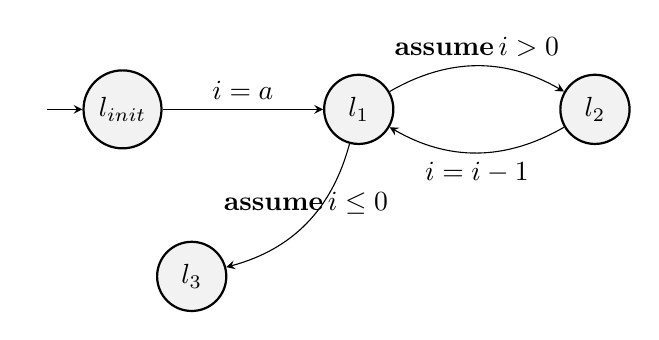
\begin{tikzpicture}
        \node[state, initial] (q1) {$l_{init}$};
        \node[state, right of=q1] (q2) {$l_1$};
        \node[state, right of=q2] (q3) {$l_2$};
        \node[state, below left of=q2] (q4) {$l_3$};
        \draw (q1) edge[above] node{$i = a$} (q2)
        (q2) edge[bend left, above] node{$\mathbf{assume} \, i > 0$} (q3)
        (q3) edge[bend left, below] node{$i = i - 1$} (q2)
        (q2) edge[bend left, above] node{$\mathbf{assume}\, i \leq 0$} (q4);
    \end{tikzpicture}
    \caption{CFG表示}
  \end{subfigure}
  \caption{程序的CFG表示示例}
  \label{fig:chap2-cfg-example}
\end{figure}

下面的定义则描述了程序的一次执行是如何组成的:

\begin{definition}
  程序$P = (L, \tau, l_0, \tmop{Var},
  \tmop{Var}_{\tmop{in}})$的格局(configuration)c是$L \times
  S$中的元素,用$(l,
  s)$表示。直观地,l是程序计数器(PC)当前的位置,而s刻画了程序中变量当前的值。
\end{definition}

\begin{definition}
  程序的一次执行(run)r是格局的一条最大序列$(l_0, s_0)
  \rightarrow (l_1, s_1) \rightarrow
  \cdots$,其中$l_0$是初始位置,且满足$\forall i \in \mathbb{N},
  \exists (l_i, \tmop{stmt}, l_{i + 1}) \in \tau, \{ s_i \} \tmop{stmt} \{
  s_{i + 1} \}$。
  
  如果r是有限的,称其为终止(terminating)的执行;否则,称为非终止(nonterminating)的执行。
  
  其中,“最大序列”指的是:若r是终止的执行,$(l_{\tmop{end}},
  s_{\tmop{end}})$是序列中的最后的格局,则应满足不存在转移$(l_{\tmop{end}},
  \tmop{stmt}, l') \in \tau$和状态$s'$,使得$\{ s_{\tmop{end}} \}
  \tmop{stmt} \{ s' \}$。
\end{definition}

终止执行的长度是一个自然数,直观上,它代表程序在实际情况下的一次运行所执行的步数(语句块的数量)。正如在引言中指出的,这可以作为一种上界指标,它对应于在程序的资源消耗模型中,任意语句的资源消耗恒为1的情况。我们可以姑且将其称为“长度上界”——不过,虽然它能准确地刻画程序的复杂度性质,却不利于进行验证。

由于工作语言\tmtextbf{Imp}中无递归,在长度上界中起决定作用的其实是程序中循环的结构,而语句块的数量等只在常数意义上对其有所影响。基于此,我们在本文中采用的是循环上界(见定义\ref{def:chap2-loop-bound})作为上界的定义,非形式化地来说,即程序的CFG表示中环路出现的次数。为此,下一节将从CFG的结构出发引入循环的概念。

\section{循环}

我们从有向图路径的角度给出自然循环的概念。在下述定义中,假设给定程序$P
= (L, \tau, l_0, \tmop{Var}, \tmop{Var}_{\tmop{in}})$。

\begin{definition}
  设$a, b \in
  L$是程序P中的两个位置,则$a$支配$b$,当且仅当$a$在所有从$l_0$到$b$的路径上。
\end{definition}

\begin{definition}
  设$t = (l, \tmop{stmt}, l') \in \tau$是程序$P$中的一条边,则$t$是$P$中的一条回边(back edge),当且仅当$l'$支配$l$。此时称$l'$是P中的一个循环头(loop header),即位置$l'$是循环头当且仅当它是某条回边的目标位置。
\end{definition}

\begin{definition}
  设$l$是$P$中的一个循环头,则$l$对应的自然循环(natural loop)是满足如下条件的一组位置$l'$的最大集合(maximal set):
  
  \begin{enumerate}
    \item $l$支配$l'$
    
    \item 存在从某个位置$l''$到$l$的一条回边,使得$l'$到$l''$有一条不经过l的路径
  \end{enumerate}
\end{definition}

本篇论文中我们也将自然循环简称为循环。自然循环的定义表明,并非CFG中的所有环路都可作为循环,从而参与上界的计算。通常,自然循环对应于实际程序中的循环结构,如C语言中的三种循环在CFG中都是自然循环。自然循环的特点是只有一个循环头作为循环的入端,可能内部有嵌套循环与分支等。为了更准确地描述程序在一次执行中所经过的循环中的实际位置,我们引入循环路径的概念:

\begin{definition}
  循环路径(loop path)是程序中的一条简单环路\footnote{即除$l_1$外,路径中不存在重复的位置}$l_1 \rightarrow l_2 \rightarrow l_3 \rightarrow \cdots \rightarrow l_{n - 1} \rightarrow l_n = l_1$,满足$l_1$是循环头,且对任意$i \in [1, n]$,$l_i$都在$l_1$的自然循环中。
\end{definition}

循环路径代表一次具体的执行在循环中可能经过的简单路径模式(pattern)。图\ref{fig:chap2-cfg-complex}是一个由实际程序翻译而来的程序,按照定义可知,$l_2$,$l_3$和$l_4$都是循环头,它们分别对应于一个自然循环,每个自然循环有一条循环路径,如表\ref{tab:chap2-loop-path}所示。

\begin{figure}
    \centering
    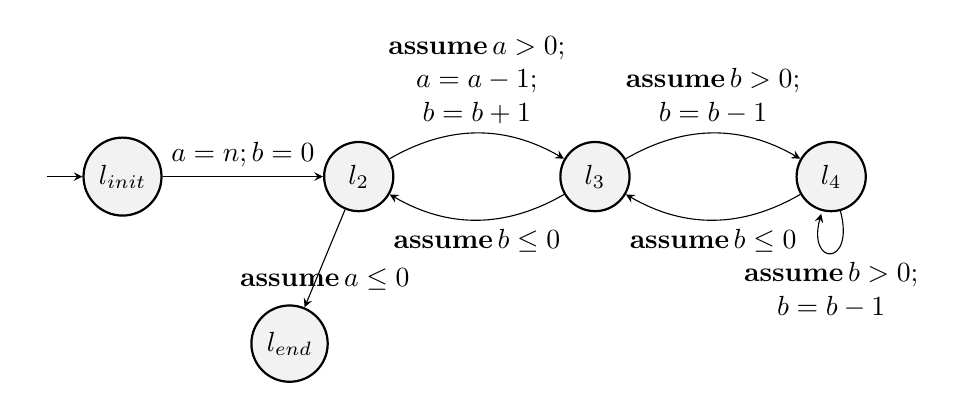
\begin{tikzpicture}[auto]
    
        \node[state, initial] (q1) {$l_{init}$};
        \node[state, right of=q1] (q2) {$l_2$};
        \node[state, right of=q2] (q3) {$l_3$};
        \node[state, right of=q3] (q4) {$l_4$};
        \node[state, below right of=q1] (q6) {$l_{end}$};
        
        \draw (q1) edge[above] node{$a = n; b = 0$} (q2)
        (q2) edge[bend left, above] node[align=center]{$\mathbf{assume} \, a > 0;$ \\ $a = a - 1;$ \\ $b = b + 1$} (q3)
        (q2) edge[below] node{$\mathbf{assume} \, a \leq 0$} (q6)
        (q3) edge[bend left, below] node{$\mathbf{assume} \, b \leq 0$} (q2)
        (q3) edge[bend left, above] node[align=center]{$\mathbf{assume}\, b > 0;$ \\ $b = b - 1$} (q4)
        (q4) edge[bend left, below] node{$\mathbf{assume}\, b \leq 0$} (q3)
        (q4) edge[loop below] node[align=center]{$\mathbf{assume}\, b > 0;$ \\ $b = b - 1$} (q4);
        
    \end{tikzpicture}
    \caption{一个实际程序}
    \label{fig:chap2-cfg-complex}
\end{figure}

\begin{table}
  \centering
  \begin{tabular}{lll}
    \toprule
    循环头 & 自然循环 & 循环路径\\
    \midrule
    $l_2$ & $\{l_2, l_3, l_4\}$ & $l_2 \rightarrow l_3 \rightarrow l_2$\\
    $l_3$ & $\{l_3, l_4\}$ & $l_3 \rightarrow l_4 \rightarrow l_3$\\
    $l_4$ & $\{l_4\}$ & $l_4 \rightarrow l_4$\\
    \bottomrule
  \end{tabular}
  \caption{图\ref{fig:chap2-cfg-complex}中的自然循环与循环路径}
  \label{tab:chap2-loop-path}
\end{table}

借助于循环路径的概念,可以很方便地从循环的角度对上界进行定义。下一节将引入本论文考虑和验证的主要对象——循环上界。

\section{上界}

这一节形式化地给出上界的定义。首先,我们需要说明何为循环路径的实例:

\begin{definition}
  令$\pi = l_1 \rightarrow l_2 \rightarrow \cdots \rightarrow l_{n - 1}
  \rightarrow
  l_1$是P中的一条循环路径,称路径v是$\pi$的一个实例,当且仅当v形如$l_1
  \rightarrow l_2 \ast l_2 \rightarrow \cdots \rightarrow l_{n - 1} \ast l_{n
  - 1} \rightarrow l_1$,其中,$l_i \ast
  l_i$表示P中任意一条从$l_i$到$l_i$,且不经过$l_1$的路径。如果v是路径p的子路径,则称p中包含实例v。
\end{definition}

直观来说,一个循环路径的实例是循环路径这一模式在一条具体路径上的实例化,或泛化(generalization)。比如,图\ref{fig:chap2-cfg-complex}的CFG中,考虑路径$l_{init} \rightarrow l_2 \rightarrow l_3 \rightarrow l_4 \rightarrow l_4 \rightarrow l_3 \rightarrow l_2 \rightarrow l_3 \rightarrow l_2 \rightarrow l_{end}$,其中包含了如下几个循环路径的实例:

\begin{enumerate}
    \item $l_2 \rightarrow l_3 \rightarrow l_2$(路径$l_2 \rightarrow l_3 \rightarrow l_2$的实例)
    \item $l_2 \rightarrow l_3 \rightarrow l_4 \rightarrow l_4 \rightarrow l_3 \rightarrow l_2 \rightarrow l_3 \rightarrow l_2$(路径$l_2 \rightarrow l_3 \rightarrow l_2$的实例)
    \item $l_4 \rightarrow l_4$(路径$l_4 \rightarrow l_4$的实例)
    \item $l_3 \rightarrow l_4 \rightarrow l_4 \rightarrow l_3$(路径$l_3 \rightarrow l_4 \rightarrow l_3$的实例)
\end{enumerate}

我们认为,如果在程序的一次执行中包含一个循环路径的实例,则可以视为相应循环的一次迭代。对任意一条循环路径,我们可以定义路径上界为一个关于输入参数的符号表达式,保证在任意情况下实例的出现数量都不超过之:

\begin{definition}
  设$\pi$是一条循环路径,则$\pi$在程序P中的路径上界(path bound)是一个$\tmop{Var}_{\tmop{in}}$上的算数表达式\footnote{终止的程序必然存在界,但不一定能用定义\ref{def:chap2-arith-expr}中定义的算数表达式类A来表示。实际上,如果把界看作是一个从输入参数到自然数的函数,它甚至不一定是可计算的。这里我们只考虑以\tmtextbf{Imp}中的简单算数表达式所能表达的上界,在下一章中提出的验证方法并不关心表达式的具体类型,因此也适用于其他类型的表达式,只要底层的安全属性检查器支持之。}$\varphi$,使得对P的所有执行$(l_0,
  s_0) \rightarrow (l_1, s_1) \rightarrow \cdots$,路径$l_0 \rightarrow l_1
  \rightarrow \cdots$所包含的$\pi$的实例的数量总是不超过$s_0
  (\varphi)$。
\end{definition}

最后,我们给出自然循环的循环上界的定义:

\begin{definition}
  \label{def:chap2-loop-bound}
  设$L_h$是程序P中的自然循环,l是其循环头,则$L_h$的(全局)循环上界(global loop bound)是一个$\tmop{Var}_{\tmop{in}}$上的算数表达式$\varphi$,使得对P的所有执行$(l_0, s_0) \rightarrow (l_1, s_1) \rightarrow \cdots$,路径$l_0 \rightarrow l_1 \rightarrow \cdots$中所包含的从l出发的所有循环路径的实例的和总是不超过$s_0 (\varphi)$。
\end{definition}

循环上界刻画了自然循环在程序中迭代的次数,这是一个全局意义下的概念,在后续的章节中我们将考虑嵌套循环情况下的循环的局部上界。最后,为了定义的完整性,对于一个程序P而言,我们可以类似地定义程序上界(program
bound)为所有循环路径实例和的上界,但在验证时,我们将把粒度限制在循环这一级。在下一章中,我们将介绍如何以程序中各自然循环的(全局的或局部的)循环上界为基础来表示程序上界,以及它们之间存在的数量关系。

\section{安全属性检查}

\label{section:chap2-safety-check}

引言部分已简述了安全属性的概念。但要形式化地定义什么是程序的规范,以及更进一步地,什么是安全属性,都需要大量的篇幅。受限于此,此处只简要说明在程序的CFG表示层面,安全属性的一种表示形式。

我们已非形式化地指出,安全属性是这样一类属性:它规定了程序在运行时,不会进入某些非预期的状态。在实际的程序中,诸如非法调用函数的参数、数组下标越界等等的行为都会导致这样的非预期状态。但是,在定义\ref{def:chap2-program}中对程序的定义,只关心了其计算层面的行为,因此我们可以只关注于程序的功能正确性(functional
correctness)。

因此,我们为定义\ref{def:chap2-program}中的程序加入一个特殊的位置$l_{\tmop{err}}$,它代表的就是程序的“错误位置”。每一个错误位置$l_{\tmop{err}}$都对应于一个安全属性,代表“程序永远不会进入位置$l_{\tmop{err}}$”。在实际的程序中,通常通过断言(assertion)来引入对程序正确性的一种规定,如C语言中的assert宏。虽然只是选定了一个特殊的位置\footnote{因为如果程序中存在多个错误位置,可以通过简单的方法将其变换为惟一的错误位置,因此下文假设程序中可以有多个错误位置},程序所有的功能正确性断言都可以转换为这种表示。比如,对于图\ref{fig:chap2-cfg-complex}中的程序,如果断言“程序一定不会终止”,则只需将代表程序终止的位置$l_{end}$视作错误位置;代码\ref{fig:chap2-cfg-assert}中的程序存在着一个断言语句,可以将其翻译为如下带有错误位置的表示:

\begin{figure}
  \begin{subfigure}[b]{.5\linewidth}
    \begin{minted}{c}
        int main() {
            int x, y;
        
            x = 0;
            y = nondet();
            while (y) {
                x = x + 1;
                y = nondet();
            }
        
            assert (x != -1);
            return 0;
        }
    \end{minted}
    \caption{带有功能正确性断言的C函数}
  \end{subfigure}
  \begin{subfigure}[b]{.5\linewidth}
    \centering
    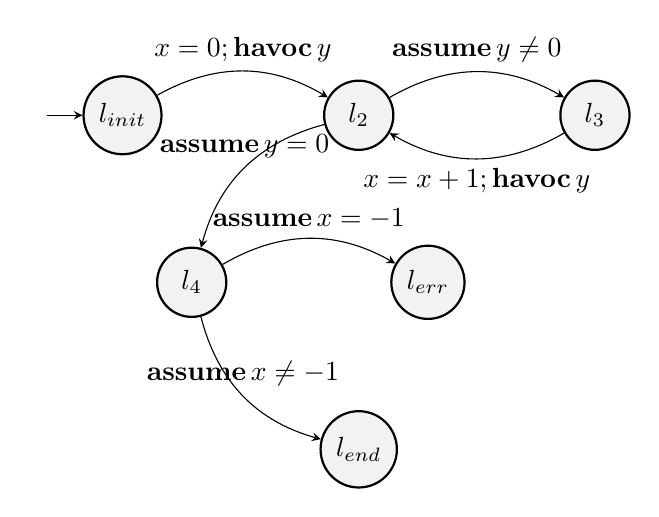
\begin{tikzpicture}[auto]
        \node[state, initial] (q1) {$l_{init}$};
        \node[state, right of=q1] (q2) {$l_2$};
        \node[state, right of=q2] (q3) {$l_3$};
        \node[state, below left of=q2] (q4) {$l_4$};
        \node[state, right of=q4] (q5) {$l_{err}$};
        \node[state, below right of=q4] (q6) {$l_{end}$};
        
        \draw (q1) edge[bend left, above] node{$x = 0; \mathbf{havoc} \, y$} (q2)
            (q2) edge[bend left, above] node{$\mathbf{assume} \, y \neq 0$} (q3)
            (q3) edge[bend left, below] node{$x = x + 1; \mathbf{havoc}\, y$} (q2)
            (q2) edge[bend right, above] node{$\mathbf{assume}\, y = 0$} (q4)
            (q4) edge[bend left, above] node{$\mathbf{assume}\, x = -1$} (q5)
            (q4) edge[bend right, above] node{$\mathbf{assume}\, x \neq -1$} (q6);
    \end{tikzpicture}
    \caption{CFG表示}
  \end{subfigure}
  \caption{带断言语句的实际程序,以及与之对应的程序CFG表示和错误位置}
  \label{fig:chap2-cfg-assert}
\end{figure}

如何进行安全属性的检查并非本篇论文关注的内容,数十年来,已经有大量的研究致力于求解此问题,如\cite{heizmann_software_2013,bakhirkin_recurrent_2016}等。虽然安全属性检查在通常意义下是一个不可判定问题,目前已有很多在实际场景中得到广泛应用的检查器能够高效地求解此问题。我们假定存在一个可靠的(sound)安全属性检查器,第三章将给出在此基础上的上界验证算法,而第四章中将给出基于Ultimate安全属性检查器的具体实现。
% !TeX root = ../main.tex

\chapter{基于安全属性检查的上界验证}

这一章将在抽象程序层面给出基于安全属性检查方法的循环上界验证算法。首先,我们将考察单一循环的上界,指出如何通过程序变换(program
transformation)将循环上界的验证问题归约到安全属性检查问题。随后,我们提出局部上界的概念,用于表示嵌套循环结构中,内层循环相对于外层循环的迭代次数,以便于更加灵活地进行验证。最后,我们以自然循环之间的嵌套关系为基础,给出程序上界的一种离散表示,并结合循环上界的验证方法,给出程序上界的整体验证算法。

\section{循环上界的验证}

\label{section:chap3-global-verif}

这一节考虑单一一个自然循环的上界验证问题。试将此问题表述如下:给定程序$P$,$P$的一个自然循环$L_h$,以及算数表达式$\varphi$,判定$\varphi$是否是$L_h$的循环上界。

我们的基本思路如下:首先采用程序变换的方式,构建一个经过调整(instrumentation)的程序$I
(P)$,使得$I
(P)$能完全模拟P的行为,且$L_h$的所有循环路径实例的出现都被计数器记录。特别的,在程序$I\left(P\right)$中加入了一个错误位置$l_{\tmop{err}}$,当且仅当循环路径实例的出现次数超过了$\varphi
(s_0)$时会进入此位置。之后,我们对程序$P'$调用安全属性检查器进行验证,如果验证通过则可以证明$\varphi$是原程序P的一个循环上界,验证不通过则可以证明$\varphi$不是原程序P的循环上界。

形式化地,设程序$P = (L, \tau, l_0, \tmop{Var},
\tmop{Var}_{\tmop{in}})$,表达式$\varphi$是关于$\tmop{Var}_{\tmop{in}}$的算数表达式,$L_h$代表以位置$l_h$为循环头的自然循环,$L'
\subseteq
L$是$L_h$中的位置集合,$\tau_{|L'}$是变迁关系在$L'$上的限制。则程序变换算法I将程序P变换为程序$I
(P) = (L \cup \{ l_{\tmop{err}}, l_{\tmop{instr}}, l_0' \}, \tau', l_0',
\tmop{Var} \cup \{ i \}, \tmop{Var}_{\tmop{in}})$,其中$i \nin
\tmop{Var}$是一个新(fresh)的变量,$l_0' \nin
L$是新的初始状态,而$\tau'$由如下的规则确定:
\begin{itemize}
  \item 对任意$(l, \tmop{stmt}, l') \in \tau$,如果$l \neq l_h \vee l'
  \nin L'$,则$(l, \tmop{stmt}, l') \in \tau'$
  
  \item 对任意$(l, \tmop{stmt}, l') \in \tau$,如果$l = l_h \wedge l'
  \in L'$,则$(l_{\tmop{instr}}, \tmop{stmt}', l') \in
  \tau'$,其中$\tmop{stmt}' \assign \textbf{assume}\, i \, \geqslant 0
  \, \textbf{;} \, \tmop{stmt}$
  
  \item $(l_h, i = i - 1, l_{\tmop{instr}}) \in \tau'$
  
  \item $(l_{\tmop{instr}}, \textbf{assume} \, i < 0, l_{\tmop{err}})
  \in \tau'$
  
  \item $(l_0', i = \varphi, l_0) \in \tau'$
\end{itemize}


非形式化地说,算法I引入了一个计数器变量i,并在程序入口处将其初始化为待验证的上界表达式;此外,每当控制流进入循环$L_h$,计数器i都将递减。如果此时计数器的值变为负,则进入错误状态$l_{\tmop{err}}$,否则继续正常运行。

图\ref{fig:global-instrumentation}形象地描述了算法I对程序的变换。

\begin{figure}
    \begin{subfigure}[b]{0.5\linewidth}
        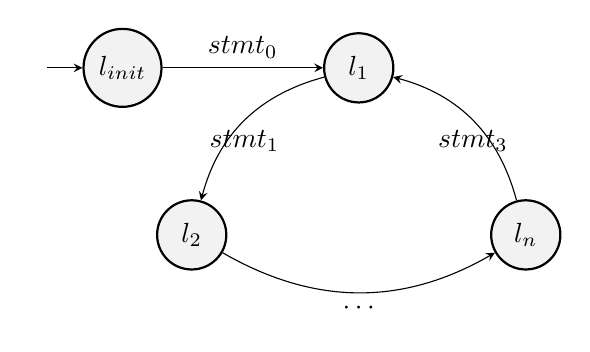
\begin{tikzpicture}
            \node[state, initial] (q0) {$l_{init}$};
            \node[state, right of=q0] (q1) {$l_{1}$};
            \node[state, below left of=q1] (q2) {$l_2$};
            \node[state, below right of=q1] (q3) {$l_n$};
            
            \path[->] 
                (q0) edge[above] node{$stmt_0$} (q1)
                (q1) edge[bend right, below] node{$stmt_1$} (q2)
                (q2) edge[bend right, below] node{$\cdots$} (q3)
                (q3) edge[bend right, below] node{$stmt_3$} (q1);
        \end{tikzpicture}
        \caption{原程序}
    \end{subfigure}
    \begin{subfigure}[b]{0.5\linewidth}
        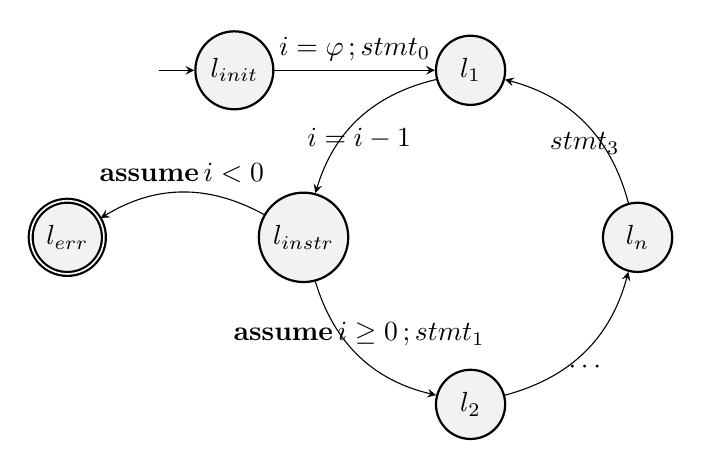
\begin{tikzpicture}
            \node[state, initial] (q0) {$l_{init}$};
            \node[state, right of=q0] (q1) {$l_1$};
            \node[state, below left of=q1] (q4) {$l_{instr}$};
            \node[state, below right of=q4] (q2) {$l_2$};
            \node[state, above right of=q2] (q3) {$l_n$};
            \node[state, left of=q4, accepting] (q5) {$l_{err}$};
            
            \path[->] 
                (q0) edge[right, above] node{$i = \varphi\,\mathbf{;}\,stmt_0$} (q1)
                (q1) edge[bend right, below] node{$i = i - 1$} (q4)
                (q4) edge[bend right, above] node{$\mathbf{assume}\, i < 0$} (q5)
                (q4) edge[bend right, above] node{$\mathbf{assume}\, i \geq 0\, \mathbf{;}\, stmt_1$} (q2)
                (q2) edge[bend right, below] node{$\cdots$} (q3)
                (q3) edge[bend right, below] node{$stmt_3$} (q1);
        \end{tikzpicture}
        \caption{变换后的程序}
    \end{subfigure}
    \caption{验证全局上界采取的程序变换示意}
    \label{fig:global-instrumentation}
\end{figure}

我们使用安全属性检查器对得到的新程序$I
(P)$进行验证。安全属性检查器可能会返回三种可能的结果:正确、错误或未知,它们分别代表程序中的错误位置不会被访问,有可能被访问,以及检查器无法证明是何种情况。我们将检查器视为黑盒进行调用,并根据其返回的结果作出如下的宣称:

\begin{lemma}
  如果安全属性检查器对程序$I
  (P)$返回“正确”,则$\varphi$是程序P中自然循环$L_h$的循环上界;如果返回“错误”,则$\varphi$不是$L_h$的循环上界。
\end{lemma}

\begin{proof}
  
  假设安全属性检查器返回“正确”,但$\varphi$不是$L_h$的循环上界,即存在P的执行$(l_0,
  s_0) \rightarrow (l_1, s_1) \rightarrow
  \cdots$,满足其中任意的位置都不是$l_{\tmop{err}}$,且$L_h$的循环路径实例出现次数大于$\varphi
  (s_0)$。
  
  根据上述程序变换的过程,$(l_0', s_0) \rightarrow (l_0, s_0')
  \rightarrow (l_1, s_1') \rightarrow \cdots$是程序$I
  (P)$的执行,其中$s_0' = s_0 [i / \varphi]$,且对任意的$j
  \geqslant 1$,如果$l_{j - 1} = l_h$且$l_{j -
  1}$是路径中循环头$l_h$的第$k$次出现,则$s_j' = s_j [i /
  \varphi - k]$,否则$s_j' = s_j [i / s_{j - 1}' (i)]$。
  
  因为$L_h$的循环路径实例出现次数大于$\varphi
  (s_0)$,而每一次实例的出现都必然经过循环头$l_h$,则存在$j
  \geqslant 1$使得$l_{j - 1} = l_h$且$l_{j -
  1}$是路径中循环头$l_h$的第$\varphi (s_0) +
  1$次出现,从而有$s_j' (i) = - 1$。
  
  由于$l_{j - 1} =
  l_h$,而根据变换的过程,$l_h$的后继只有$l_{\tmop{instr}}$,此外程序的执行是最大序列,在$l_j$处根据定义\ref{def:chap2-semantics}中假设断言语句的语义,$\{
  s_j' \} \textbf{assume} \, i \geqslant 0 \{ s_{j + 1}'
  \}$不成立,但$\{ s_j' \} \textbf{assume} \, i < 0 \{ s'_j
  \}$成立,因此必有$(l_j, s_j') \rightarrow (l_{\tmop{err}},
  s_j')$,即错误位置被访问。这与安全属性检查器的结果矛盾。所以$\varphi$是$L_h$的循环上界。
  
  同理,可以证明当检查器返回“错误”时,$\varphi$不是$L_h$的循环上界。
\end{proof}

引理1说明安全属性检查器在经过调整的程序$I
(P)$上给出的结果,与待验证的上界$\varphi$在原程序P中是否成立是一致的。算法\ref{alg:global-verif}给出了这一算法的伪代码。

\renewcommand{\algorithmicrequire}{\textbf{输入:}\unskip}
\renewcommand{\algorithmicensure}{\textbf{输出:}\unskip}
\renewcommand{\algorithmiccomment}[1]{\hfill// #1}
\begin{algorithm}
  \caption{验证循环的全局上界}
  \label{alg:global-verif}
  %\small
  \begin{algorithmic}
    \REQUIRE 程序$P$,$P$中的自然循环$L_h$,上界表达式$\phi$
    \ENSURE $\phi$是否是$L$的全局上界

    \STATE $(L, \tau, l_0, Var, Var_{in}) \leftarrow P$
    \STATE $Var' \leftarrow Var \cup \{i\}$ \COMMENT i是不在Var中的变量
    \STATE $\tau' \leftarrow \{\}$
    \STATE $l \leftarrow$ loop header of $L_h$
    \STATE create new location $l_{err}, l_{instr}$ and $l_0'$
    \STATE add $(l_0', l_0, i = \phi)$ to $\tau'$
    \STATE add $(l, l_{instr}, i = i - 1)$ to $\tau'$
    \STATE add $(l_{instr}, l_{err}, \mathbf{assume}\, i < 0)$ to $\tau'$
    \FORALL{$(l_1, l_2, s) \in \tau$ where $l_1 = l$}
        \STATE add $(l_{instr}, l_2, \mathbf{assume}\, i \geq 0\, \mathbf{;}\, s)$ to $\tau'$
    \ENDFOR
    \FORALL{$(l_1, l_2, s) \in \tau$ where $l_1 \neq l$}
        \STATE add $(l_1, l_2, s)$ to $\tau'$ 
    \ENDFOR
    \STATE $P' \leftarrow (L, \tau', l_0', Var', Var_{in})$
    
    \STATE call safety checker on $P'$ \COMMENT{调用安全属性检查器}
    \IF{safety check succeeded}
        \RETURN \TRUE
    \ELSIF{safety check failed}
        \RETURN \FALSE
    \ELSIF{safety check has no result}
        \RETURN unknown
    \ENDIF

  \end{algorithmic}
\end{algorithm}

\section{嵌套循环局部上界的验证}

这一节考虑一种特殊的情况,即在嵌套循环中,内层循环的上界应该如何验证。根据定义,一个循环的上界是其循环路径实例在全局意义下的出现次数的界。所谓全局意义,指的是在程序的一次执行中,将所有实例的出现次数一同进行计数,最终得到总和。实际程序中,嵌套循环是非常常见的结构。所谓嵌套,可以很简单地进行定义如下:外层循环$L_{\tmop{out}}$嵌套内层循环$L_{\tmop{inner}}$,当且仅当$L_{\tmop{inner}}$的循环头在自然循环$L_{\tmop{out}}$中。

对于存在于嵌套中的内层循环,当然也可以通过上一节的方法验证上界,这种方法能较好地适用于内外循环关联不强的情况。比如,代码\ref{listing:chap3-indep-nested}中,函数fun有一个两层的循环,但它们并不会使用相同的变量。实际上,内层循环虽然语法上嵌套在外层循环之中,它们的语义却是相互独立的。内层循环的上界是$max(b, 0)$\footnote{这里max(a,b)是条件表达式$a>b\,?\,a:b$的简写,下文同。因为在本文的形式化中控制流都由流图表示,因此条件表达式不在定义\ref{def:chap2-arith-expr}中。实际实现支持此类表达式。},与外层循环的迭代次数无关。

\begin{listing}
\begin{minted}
[
frame=lines,
framesep=2mm,
baselinestretch=1,
fontsize=\footnotesize,
linenos
]{c}
void fun(int a, int b) {
    while (a >= 2) {
        a = a - 1;
        while (b > 0) {
            b--;
        }
    }
}
\end{minted}
\caption{一个含有相互独立的嵌套循环的C语言函数}
\label{listing:chap3-indep-nested}
\end{listing}   

但是,更常见的是诸如代码\ref{listing:chap3-dep-nested}的程序。在这里,每当外层循环迭代一次,内层循环就随之迭代i次,故其总的迭代次数是$1
+ 2 + \ldots + n = \frac{n (n +
1)}{2}$,这也是内层循环的上(确)界:

\begin{listing}
\begin{minted}
[
frame=lines,
framesep=2mm,
baselinestretch=1,
fontsize=\footnotesize,
linenos
]{c}
void fun(int n) {
    for (int i = 1; i <= n; i++) {
        int j = i;
        while (j > 0) {
            j--;
        }
    }
}
\end{minted}
\caption{一个含有非独立的嵌套循环的C语言函数}
\label{listing:chap3-dep-nested}
\end{listing}

在这里,我们实际上是通过考察在外层循环的两次迭代之间内层循环出现次数的上界来解决循环上界的问题。局部上界在很多情况下相对于全局的循环上界而言更加直观,也更容易由自动上界求解器或者人工计算得到,因此,支持局部上界的验证是有必要的。一旦算出程序中所有循环的全局或局部上界,我们可以通过简单的算数运算求得程序的上界,这将在下一节进行说明。这里,我们首先给出局部上界的形式化定义:

\begin{definition}
  设$L_{\tmop{outer}}$和$L_{\tmop{inner}}$是程序P中的自然循环,$l_{\tmop{outer}}$和$l_{\tmop{inner}}$是其循环头,则$L_{\tmop{inner}}$相对于$L_{\tmop{outer}}$的局部循环上界(local
  loop
  bound)是一个$\tmop{Var}_{\tmop{in}}$上的算数表达式$\varphi$,使得对P的所有执行$r
  = (l_0, s_0) \rightarrow (l_1, s_1) \rightarrow \cdots$以及路径$l_0
  \rightarrow l_1 \rightarrow
  \cdots$中所包含的所有$L_{\tmop{outer}}$的循环路径实例$v =
  l_{\tmop{outer}} \rightarrow l_1' \rightarrow l_2' \rightarrow \cdots
  \rightarrow
  l_{\tmop{outer}}$,路径v中$L_{\tmop{inner}}$的所有循环路径的实例的和总是不超过$s_{\tmop{outer}}
  (\varphi)$,其中$(l_{\tmop{outer}},
  s_{\tmop{outer}})$是r中v的起始位置对应的格局。
\end{definition}

我们可以类似地给出一种程序变换的方法,将局部上界的验证归约为安全属性的验证。设程序$P
= (L, \tau, l_0, \tmop{Var},
\tmop{Var}_{\tmop{in}})$,表达式$\varphi$是关于$\tmop{Var}_{\tmop{in}}$的算数表达式,$L_{\tmop{outer}}$是以位置$l_{\tmop{outer}}$为循环头的自然循环,$L_{\tmop{inner}}$是以位置$l_{\tmop{inner}}$为循环头的自然循环。则程序变换算法$I_{\tmop{nested}}$将程序P变换为程序$I_{\tmop{nested}}
(P) = (L \cup \{ l_{\tmop{err}}, l_{\tmop{nested}}, l_{\tmop{instr}} \},
\tau', l_0, \tmop{Var} \cup \{ i \}, \tmop{Var}_{\tmop{in}})$,其中$i \nin
\tmop{Var}$是一个新的变量,$\tau'$由如下的规则确定:
\begin{itemize}
  \item 对任意$(l, \tmop{stmt}, l') \in \tau$,如果$l = l_{\tmop{inner}}
  \wedge l' \in L_{\tmop{inner}}$,则$(l_{\tmop{instr}}, \tmop{stmt}', l')
  \in \tau'$,其中$\tmop{stmt}' \assign \textbf{assume} \, i \,
  \geqslant 0 \textbf{;} \, \tmop{stmt}$
  
  \item 对任意$(l, \tmop{stmt}, l') \in \tau$,如果$l = l_{\tmop{outer}}
  \wedge l' \in L_{\tmop{outer}}$,则$(l_{\tmop{nested}}, \tmop{stmt},
  l_{}') \in \tau'$
  
  \item 对其余$(l, \tmop{stmt}, l') \in \tau$有$(l, \tmop{stmt}, l') \in
  \tau'$
  
  \item $(l_{\tmop{inner}}, i = i - 1, l_{\tmop{instr}}) \in \tau'$
  
  \item $(l_{\tmop{instr}}, \textbf{assume} \, i < 0, l_{\tmop{err}})
  \in \tau'$
  
  \item $(l_{\tmop{outer}}, i = \varphi, l_{\tmop{nested}}) \in \tau'$
\end{itemize}


图\ref{fig:local-instrumentation}直观地描述了$I_{\tmop{nest}} (P)$的结构。

\begin{figure}
    \begin{subfigure}[b]{0.5\linewidth}
        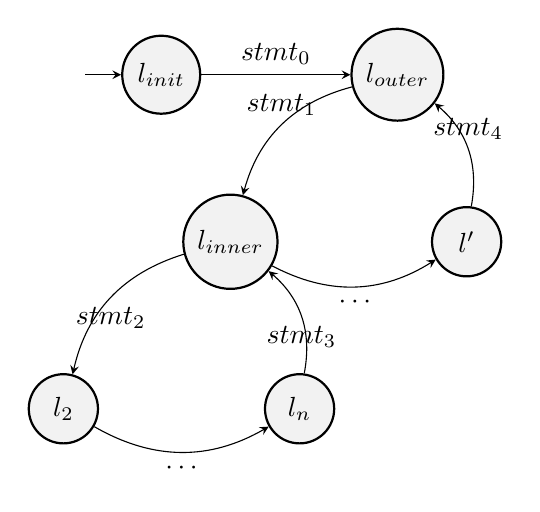
\begin{tikzpicture}
            \node[state, initial] (q0) {$l_{init}$};
            \node[state, right of=q0] (qo) {$l_{outer}$};
            \node[state, below left of=qo] (q1) {$l_{inner}$};
            \node[state, below left of=q1] (q2) {$l_2$};
            \node[state, right of=q2] (q3) {$l_n$};
            \node[state, right of=q1] (q4) {$l'$};
            
            \path[->] 
                (q0) edge[above] node{$stmt_0$} (qo)
                (qo) edge[bend right, above] node{$stmt_1$} (q1)
                (q1) edge[bend right, below] node{$stmt_2$} (q2)
                (q2) edge[bend right, below] node{$\cdots$} (q3)
                (q3) edge[bend right, below] node{$stmt_3$} (q1)
                (q1) edge[bend right, below] node{$\cdots$} (q4)
                (q4) edge[bend right, above] node{$stmt_4$} (qo);
        \end{tikzpicture}
        \caption{原程序}
    \end{subfigure}
    \begin{subfigure}[b]{0.5\linewidth}
        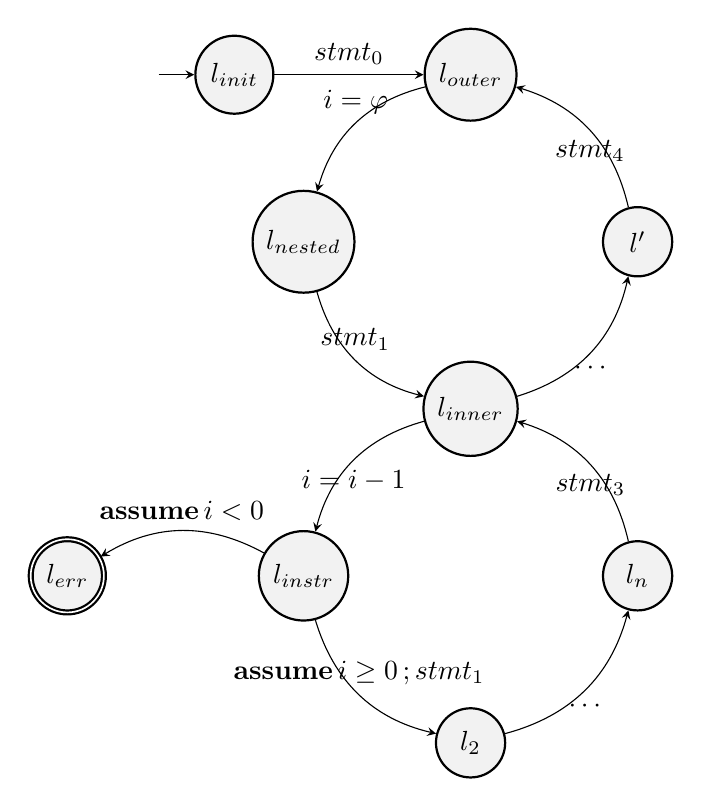
\begin{tikzpicture}
            \node[state, initial] (q0) {$l_{init}$};
            \node[state, right of=q0] (qo) {$l_{outer}$};
            \node[state, below left of=qo] (qn) {$l_{nested}$};
            \node[state, below right of=qn] (q1) {$l_{inner}$};
            \node[state, below left of=q1] (q4) {$l_{instr}$};
            \node[state, below right of=q4] (q2) {$l_2$};
            \node[state, above right of=q2] (q3) {$l_n$};
            \node[state, left of=q4, accepting] (q5) {$l_{err}$};
            \node[state, above right of=q1] (q6) {$l'$};
            
            \path[->] 
                (q0) edge[above] node{$stmt_0$} (qo)
                (qo) edge[bend right, above] node{$i = \varphi$} (qn)
                (qn) edge[bend right, above] node{$stmt_1$} (q1)
                (q1) edge[bend right, below] node{$i = i - 1$} (q4)
                (q1) edge[bend right, below] node{$\cdots$} (q6)
                (q6) edge[bend right, below] node{$stmt_4$} (qo)
                (q4) edge[bend right, above] node{$\mathbf{assume}\, i < 0$} (q5)
                (q4) edge[bend right, above] node{$\mathbf{assume}\, i \geq 0\, \mathbf{;}\, stmt_1$} (q2)
                (q2) edge[bend right, below] node{$\cdots$} (q3)
                (q3) edge[bend right, below] node{$stmt_3$} (q1);
        \end{tikzpicture}
        \caption{变换后的程序}
    \end{subfigure}
    \caption{验证局部上界采取的程序变换示意}
    \label{fig:local-instrumentation}
\end{figure}

和\ref{section:chap3-global-verif}节中的做法类似,我们调用安全属性检查器对$I_{\tmop{nest}}
(P)$进行检查。我们同样给出这一方法的可靠性证明:

\begin{lemma}
  如果安全属性检查器对程序$I_{\tmop{nested}}
  (P)$返回“正确”,则$\varphi$是程序P中循环$L_{\tmop{inner}}$相对于$L_{\tmop{outer}}$的循环上界;如果返回“错误”,则$\varphi$不是循环$L_{\tmop{inner}}$相对于$L_{\tmop{outer}}$的循环上界。
\end{lemma}

\begin{proof}
  
  
  假设安全属性检查器返回的结果是“正确”,即错误位置$l_{\tmop{err}}$不会被访问。如果$\varphi$不是循环$L_{\tmop{inner}}$相对于$L_{\tmop{outer}}$的循环上界,则存在$L_{\tmop{outer}}$的实例$v
  = (l_{\tmop{outer}}, s_0) \rightarrow (l_1, s_1) \rightarrow (l_2, s_2)
  \rightarrow \cdots \rightarrow (l_{\tmop{outer}},
  s_n)$,使得$L_{\tmop{inner}}$的实例在其中的出现次数大于$s_0
  (\varphi)$。
  
  由于$L_{\tmop{inner}}$嵌套于$L_{\tmop{outer}}$,$l_{\tmop{inner}}$在$L_{\tmop{outer}}$中,所以$l_{\tmop{outer}}$支配$l_{\tmop{inner}}$。根据程序变换$I_{\tmop{nested}}$的定义,$v'
  = (l_{\tmop{outer}}, s_0) \rightarrow (l_{\tmop{nested}}, s_{\tmop{nested}})
  \rightarrow (l_1, s_1') \rightarrow (l_2, s_2') \rightarrow \cdots
  \rightarrow (l_{\tmop{outer}}, s_m')$是$I_{\tmop{nested}}
  (P)$中的路径,其中$s_{\tmop{nested}} = s_0 [i / s_0
  (\varphi)]$,且对任意的$j > 1$,如果$l_{j - 1} =
  l_{\tmop{inner}}$且$l_{j -
  1}$是路径v中循环头$l_{\tmop{inner}}$的第$k$次出现,则$s_j' =
  s_j [i / s_0 (\varphi) - k]$,否则$s_j' = s_j [i / s_{j - 1}' (i)]$。
  
  和引理1的证明类似,我们可以证明,由于路径v中$L_{\tmop{inner}}$的实例数量大于$s_0
  (\varphi)$,则必有第$s_0 (\varphi) +
  1$次的出现,从而存在一个格局$(l_{\tmop{instr}}, s)$使得$s (i)
  = - 1$;由于此时$\{ s \} \textbf{assume} \, i \, \geqslant 0 \{ s
  \}$不成立,下一个格局必然是$(l_{\tmop{err}},
  s)$。这与安全属性检查器的结果矛盾。因此,$\varphi$是循环$L_{\tmop{inner}}$相对于$L_{\tmop{outer}}$的循环上界。
  
  同理,可以证明当安全属性检查器返回“错误”时,$\varphi$不是循环$L_{\tmop{inner}}$相对于$L_{\tmop{outer}}$的循环上界。
\end{proof}

算法\ref{alg:local-verif}给出了嵌套循环的局部上界验证的伪代码:

\begin{algorithm}[ht]
  \caption{验证循环的局部上界}
  \label{alg:local-verif}
  %\small
  \begin{algorithmic}
    \REQUIRE 程序$P$,外层循环$L_o$,内层循环$L_i$上界表达式$\phi$
    \ENSURE $\phi$是否是$L_i$相对于$L_o$的局部上界

    \STATE $(L, \tau, l_0, Var, Var_{in}) \leftarrow P$
    \STATE $Var' \leftarrow Var \cup \{i\}$ \COMMENT i是不在Var中的变量
    \STATE $\tau' \leftarrow \{\}$
    
    \STATE $l_o \leftarrow$ loop header of $L_o$
    \STATE $l_i \leftarrow$ loop header of $L_i$
    
    \STATE create new location $l_{err}, l_{instr}$ and $l_{nested}$
    \STATE add $(l_o, l_{nested}, i = \phi)$ to $\tau'$
    \STATE add $(l_i, l_{instr}, i = i - 1)$ to $\tau'$
    \STATE add $(l_{instr}, l_{err}, \mathbf{assume}\, i < 0)$ to $\tau'$
    \FORALL{$(l_1, l_2, s) \in \tau$ where $l_1 = l_i$}
        \STATE add $(l_{instr}, l_2, \mathbf{assume}\, i \geq 0\, \mathbf{;}\, s)$ to $\tau'$
    \ENDFOR
    \FORALL{$(l_1, l_2, s) \in \tau$ where $l_1 = l_o$}
        \STATE add $(l_{nested}, l_2, s)$ to $\tau'$
    \ENDFOR
    \FORALL{$(l_1, l_2, s) \in \tau$ where $l_1 \neq l_i$ and $l_1 \neq l_o$}
        \STATE add $(l_1, l_2, s)$ to $\tau'$ 
    \ENDFOR
    \STATE $P' \leftarrow (L, \tau', l_0', Var', Var_{in})$
    
    \STATE call safety checker on $P'$ \COMMENT{调用安全属性检查器}
    \IF{safety check succeeded}
        \RETURN \TRUE
    \ELSIF{safety check failed}
        \RETURN \FALSE
    \ELSIF{safety check has no result}
        \RETURN unknown
    \ENDIF

  \end{algorithmic}
\end{algorithm}

\section{程序的上界证明结构及其验证}

前两小节考察的是单一的自然循环,并分别给出了全局和局部意义下上界的验证算法。对于程序而言,我们关心其整体的上界。正如在上一章中指出的,如果以程序中所有循环路径实例出现的次数的和作为程序上界,
粒度会过于粗糙,也无法直接用归约到安全属性检查问题的方法来解决。在这一节中,我们提出将程序中每个循环的上界进行组合,共同构成一个证明结构(proof
structure\cite{gulwani_speed_2009}),证明结构经过运算可对应于一个程序的上界。我们给出一个简单的转换方法,最后结合上述单一循环的验证算法,给出证明结构的验证策略。

证明结构的定义如下:

\begin{definition}
  \label{def:chap3-proof-structure}
  令程序$P = (L, \tau, l_0, \tmop{Var},
  \tmop{Var}_{\tmop{in}})$,设$\tmop{Loop}$是P中所有自然循环的集合,则P的证明结构是一个二元组$(B,
  S)$,其中映射$B \in \tmop{Loop} \rightarrow
  A$将循环映射为其上界,映射$S \in \tmop{Loop} \rightarrow
  \tmop{Loop} \cup \{ \tmop{global}
  \}$将循环映射为其所在的外层嵌套循环,或是一个特殊的符号“global”。此外,满足由S生成的有向图是无环的。
\end{definition}

证明结构实际上为程序中的每一个循环$L_h$给出了两份信息:$L_h$的上界,以及此上界的作用域(scope)。这里所说的作用域,类似于实际程序中变量的作用域,但不是表示生命周期,而是表示映射B给定的上界是相对于哪一个外层循环而言的。如果是给定的上界是全局的循环上界,我们用符号“global”进行表示。

正如上界不是唯一的,程序的证明结构也不是唯一的,但是每一证明结构都对应于一个上界。可以通过如下的递归函数Bound计算每个循环的全局上界:

\begin{equation}
    Bound(L_h) = \left\{ \begin{array}{ll}
       B(L_h) & S(L_h) = "global"\\
       Bound(L_{nested}) \times B(L_h) & S(L_h) = L_{nested}
     \end{array} \right.
\end{equation}

由于证明结构是无环的,上述递归函数Bound总是会终止。直观上,这对应于在实际程序中,循环的嵌套总是有限的。

最后,程序P的上界即为:

\begin{equation}
\sum_{L_h \in Loop} Bound(L_h)
\end{equation}

这里,我们结合循环上界的验证算法提出证明结构的验证算法,算法\ref{alg:chap3-proof-structure}给出了其伪代码:和本章前两节的思路类似,对每个自然循环,我们通过程序变换引入一个计数器变量,并在作用域起始的位置将其初始化为假定的上界表达式;此外在循环内部插入赋值语句,使计数器递减,并在计数器变为负时进入错误位置。

在下一章中,我们将介绍如何由用户的输入得到证明结构,以及在实际场景的策略与实现。

\begin{algorithm}[ht]
  \caption{证明结构的验证算法}
  \label{alg:chap3-proof-structure}
  \begin{algorithmic}
    \REQUIRE 程序$P$,证明结构$(B, S)$
    \ENSURE $(B, S)$是否成立

    \STATE $(Loc, \tau, l_0, Var, Var_{in}) \leftarrow P$
    \STATE $Var' \leftarrow Var$
    \FORALL{natural loop $L$ in $P$}
        \STATE add a fresh variable $i_L$ to $Var'$ \COMMENT{为每一个循环创建计数器变量}
    \ENDFOR
    
    \STATE iter $\leftarrow$ the preorder iterator of all natural loops in $P$ 
    \STATE $\tau' \leftarrow \{\}$
    
    \WHILE{iter.hasNext}
        \STATE $L \leftarrow$ iter.next     \COMMENT{对所有自然循环按照嵌套关系进行前序遍历}
        \STATE $l \leftarrow$ loop header of $L$
        \STATE $stmt \leftarrow \{\}$ \COMMENT{下类似局部上界的程序变换方法}
        \FORALL{natural loop $L'$ such that $S(L')=L$}
            \STATE add $i_{L'} = B(L')$ to $stmt$
        \ENDFOR
        \STATE create new locations $l_{L, instr}$ and $l_{L, err}$
        \STATE add $(l, l_{L, instr}, join(stmt))$ to $\tau'$
        \STATE add $(l_{L, instr}, l_{L, err}, \mathbf{assume} \, i_L < 0)$ to $\tau'$
        \FORALL{$(l_1, l_2, s) \in \tau$ where $l_1 = l$}
            \STATE add $(l_{L, instr}, l_2, \mathbf{assume}\, i_L \geq 0\,\mathbf{;}\,s)$ to $\tau'$ 
        \ENDFOR
    \ENDWHILE
    
    \STATE $global \leftarrow \{\}$ \COMMENT{下类似全局上界的程序变换方法}
    \FORALL{natural loop $L'$ such that $S(L')="global"$}
        \STATE add $i_{L'} = B(L')$ to $global$
    \ENDFOR
    \FORALL{$(l_{init}, l', s) \in \tau$}
        \STATE add $(l_{init}, l', join(global)\,\mathbf{;}\,s)$ to $\tau$
    \ENDFOR
    \FORALL{$(l_1, l_2, s) \in \tau$ where $l_1$ is not loop header and $l_1 \neq l_{init}$}
        \STATE add $(l_1, l_2, s)$ to $\tau'$
    \ENDFOR
    \STATE $P' \leftarrow (L, \tau', l_0', Var', Var_{in})$
    
    \STATE call safety checker on $P'$ \COMMENT{调用安全属性检查器}
    \IF{safety check succeeded}
        \RETURN \TRUE
    \ELSIF{safety check failed}
        \RETURN \FALSE
    \ELSIF{safety check has no result}
        \RETURN unknown
    \ENDIF
  \end{algorithmic}
\end{algorithm}

% !TeX root = ../main.tex

\chapter{实现}

这一章将描述我们提出的上界验证算法的具体实现。我们的实现主要是基于\texttt{Ultimate}这一模块化的程序分析套件,并结合C语言的标注语言ACSL的输入格式,以及程序验证中间语言Boogie的已有技术。本章先简要介绍相关的工具,然后对算法的实现进行描述。

\section{\texttt{Ultimate} 程序分析套件概述}

\texttt{Ultimate}程序分析套件\cite{heizmann_software_2013, heizmann_termination_2014,chen_advanced_2018}是由弗莱堡大学的学者和研究人员开发和维护的一套工具,由Java编写。它也可以被认为是一个用于开发程序分析工具的框架,采用模块化的插件(plugin)系统,由一个个的插件实现和提供不同的程序分析方法。这些插件能实现从源代码解析、程序表示的转化到静态分析的一系列功能,而通过将这些插件相互组合为工具链(toolchain),可以完成非常复杂的程序分析任务。作为程序验证工具而言,\texttt{Ultimate}涵盖了安全属性检查\cite{heizmann_software_2013}、终止性分析\cite{heizmann_termination_2014}、模型检测、并发程序验证等主要领域的需求,实现了大量的主流算法。

\texttt{Ultimate}可以接受多种语言的程序,但最主要的源语言是C语言。我们可以编制一个工具链,使用\texttt{Ultimate}验证C语言程序的安全属性。图\ref{fig:ultimate-example}比较直观地展示了主要插件之间的关系。

\tikzstyle{process} = [rectangle, minimum width=3cm, minimum height=1cm, text centered, draw=black]

\begin{figure}
    \centering
    \begin{tikzpicture}
        \node (pro1) [process] {ACSL标注的C语言文件};
        \node (pro2) [process, below of=pro1] {C抽象语法树};
        \node (pro3) [process, below of=pro2] {Boogie中间表示};
        \node (pro4) [process, below of=pro3] {控制流图};
        \node (pro5) [process, below of=pro4] {验证结果或反例};
        \draw (pro1) -- node [left] {CDTParser} (pro2);
        \draw (pro2) -- node [left] {CACSL2BoogieTranslator} (pro3);
        \draw (pro3) -- node [left] {RCFGBuilder} (pro4);
        \draw (pro4) -- node [left] {TraceAbstraction} (pro5);
    \end{tikzpicture}
    \caption{\texttt{Ultimate}框架中,进行C语言程序安全属性检查时的工具链中各插件的关系,以及过程中的中间表示}
    \label{fig:ultimate-example}
\end{figure}

\texttt{Ultimate}会首先对C语言进行语法解析(插件CDTParser),得到抽象语法树,随后通过翻译过程,将其转换为Boogie这一中间表示(插件CACSL2BoogieTranslator)。在将Boogie程序转换为等价的CFG后(插件RCFGBuilder),最终进行以路径抽象(插件TraceAbstraction)为基础的安全属性检查过程\cite{heizmann_traces_2015}。

其中,Boogie\cite{leino_this_2016}是由微软提出的一种验证中间语言(intermediate verification language),类似于一般的IR,它的作用是简化高级语言验证器的开发。开发者可以实现从高级语言及其规范到Boogie的翻译,由Boogie求解器完成后续的验证。在此不赘述Boogie的语法,只给出以下代码\ref{listing:chap4-boogie-example}中的程序作为例子,从中可以看出,Boogie作为一门语言,在保留一般的命令式程序的框架的基础下保持简洁,删减了高级语言面向用户的若干特性。另外,Boogie中采用断言语句\textbf{assert} $\phi$来指定程序中的错误状态,这和\textbf{Imp}中使用独立的错误位置来代表安全属性的做法类似但稍有不同,不过这两种表示之间的对应关系是直观的。

\begin{listing}[ht]
\begin{minted}
[
frame=lines,
framesep=2mm,
baselinestretch=1,
fontsize=\footnotesize,
linenos
]{text}
procedure main()
{
  var n, p: int;

  assume p != 0;
  while (n >= 0) {
    assert(p != 0);
    if (n == 0) {
      p := 0;
    }
    n := n - 1;
  } 
}

\end{minted}
\caption{在Boogie语言中表示的简单函数以及对其的规范}
\label{listing:chap4-boogie-example}
\end{listing}

为了在C语言中表示对程序行为的规范,\texttt{Ultimate}允许输入程序在ANSI C的基础上使用ACSL进行标注。ACSL全称ANSI/ISO C Specification Language,是对C语言程序的行为进行规范的一种DSL,最早用于Frama-C\cite{kirchner_frama-c_2015}C语言程序分析套件中。ACSL可以表达丰富的规范,包括一般的行为正确性,以及和C语言中涉及的一些低级的机器细节相关的规范。代码\ref{listing:chap4-acsl-example}中的程序是一个用ACSL进行标注后的简单程序,其中,ACSL标注存在于C语言的注释之中,它既可以出现在函数定义之前,也可以出现在循环结构之前。

\begin{listing}

\begin{minted}
[
frame=lines,
framesep=2mm,
baselinestretch=1,
fontsize=\footnotesize,
linenos
]
{c}
/*@
  requires \valid(a+(0..n-1));

  assigns  a[0..n-1];

  ensures
  \forall integer i;
    0 <= i < n ==> a[i] == 0;
*/
void set_to_0(int* a, int n){
  int i;

  /*@
    loop invariant 0 <= i <= n;
    loop invariant
    \forall integer j;
      0 <= j < i ==> a[j] == 0;
    loop assigns i, a[0..n-1];
    loop variant n-i;
  */
  for(i = 0; i < n; ++i)
    a[i] = 0;
}
\end{minted}

\caption{使用ACSL标注的C语言程序示例}
\label{listing:chap4-acsl-example}
\end{listing}

\section{上界算法的实现}

\subsection{对ACSL的扩展}

ACSL中并没有能表达上界的语法结构,为了让用户能方便地在源文件中指定循环上界,我们对ACSL的语法进行了扩展,引入了如下的循环上界语句:

\[
\mathbf{loop} \, \{name\} \,\mathbf{bound} \,  \phi \, \{\mathbf{scope} \, nested\}
\]

循环上界语句和不变式语句一样,只能出现在循环之前,并对此循环的性质进行说明。其中,$\phi$是上界的符号表达式;\textit{name}是一个标识符,相当于给当前循环打上标签或起的名称;\textit{nested}也是一个标识符,它是当前循环所在的某个嵌套循环的名称,代表的是当前循环的上界的作用域。后者的存在是为了解决实际程序中可能出现的多层嵌套的情况。\textit{name}和\textit{nested}都是可选的。如果不指定\textit{nested},则对应于定义\ref{def:chap3-proof-structure}中的“global”作用域,即指定的是全局意义下的循环上界。例如,代码\ref{listing:chap4-acsl-bound}中的程序中有嵌套循环,我们分别用ACSL对其进行了标注。

\begin{listing}

\begin{minted}
[
frame=lines,
framesep=2mm,
baselinestretch=1,
fontsize=\footnotesize,
linenos
]{c}

void while2(int a, int b, int c) {
  a = b;
  //@ loop l1 bound max(b, 0);
  while (a >= 1) {
    c = b;
    //@ loop l2 bound max(b, 1) scope l1;
    while (1) {
      if (c >= 1) {
        c = c - 1;
      }
      else if (0 >= c) {
        a = a - 1;
        break;
      }
      else
        return;
    }
  }
}

\end{minted}
\caption{一个使用ACSL扩展对上界进行标注的C语言程序}
\label{listing:chap4-acsl-bound}
\end{listing}

我们修改了\texttt{Ultimate}框架的前端部分以支持新的语法,并加入了检测步骤确保语句中作用域的嵌套是合法的,即不会形成环路。显然,如果程序中每个自然循环都进行了标注,并通过检查,所得到的标注语句构成了一个证明结构。

\subsection{扩展语法的翻译}

我们沿着上一章证明结构的验证思路,实现了从C语言到Boogie的翻译过程的修改。假设每个自然循环$L$都有唯一的上界标注,这意味着一个上界表达式$\phi_L$,以及可选的名称$N_L$和作用域标识$S_L$。将ACSL标注翻译为Boogie的过程和C语言到Boogie的翻译过程紧密相连,我们假设\textbf{Translate}是C语言的翻译过程,给定一个C语言函数它返回对应的Boogie函数。

ACSL扩展部分的翻译例程如算法\ref{alg:chap4-c-to-boogie}所示。我们将翻译分为两个步骤:首先对循环进行后序遍历,将每个循环需要额外添加到作用域(或函数)入口处以及循环体入口处的语句分别记录在变量Reset(或Global)和Body中。接着,我们调用\textbf{Translate}完成函数的翻译,并在得到的新函数$P'$中插入上述语句。

\begin{algorithm}
    \begin{algorithmic}
        \REQUIRE C语言函数定义$P$
        \ENSURE Boogie函数定义$P'$
        \STATE Global $\leftarrow \{\}$ \COMMENT Global是语句的集合
        \STATE Reset $\leftarrow \{\}$ \COMMENT Reset是从循环到语句的映射
        \STATE Body $\leftarrow \{\}$ \COMMENT Body是从循环到语句的映射
        
        \STATE iter $\leftarrow$ $P$中所有自然循环的后序遍历迭代器
        \WHILE{$iter.hasNext$}
        
            \STATE L $\leftarrow$ $iter.next$
            
            \IF{$S_L = "global"$}
                \STATE $Global.add(i_L = \phi_L)$
            \ELSE
                \STATE $Reset(Name2Loop(S_L)).add(i_L = \phi_L)$
            \ENDIF
            \STATE $Body(L).add(i_L = i_L - 1; assert(i_L \geq 0))$
            \STATE $Body(L).add(Reset(L))$
        \ENDWHILE
        
        \STATE 忽略$P$中上界标注,调用\textbf{Translate}将$P$翻译为Boogie函数$P'$
        \STATE 为$P$中所有自然循环$L$在$P'$中声明整型变量$i_L$
        \FORALL{自然循环$L \in P$}
            \STATE 将$Body(L)$加到$P'$中$L$对应的循环头之后
        \ENDFOR
        \STATE 将Global中的语句加到$P'$初始位置之后
        \RETURN $P'$
    \end{algorithmic}
    \caption{带ACSL上界标注的C语言函数的翻译流程}
    \label{alg:chap4-c-to-boogie}
\end{algorithm}
        
以代码\ref{listing:chap4-acsl-bound}中的C语言函数为例,翻译后得到的Boogie函数如代码\ref{listing:chap4-acsl-bound-boogie}所示。

\begin{listing}
\caption{翻译代码\ref{listing:chap4-acsl-bound}得到的Boogie程序}
\label{listing:chap4-acsl-bound-boogie}
\begin{minted}
[
frame=lines,
framesep=2mm,
baselinestretch=1,
fontsize=\footnotesize,
linenos
]{text}
implementation while2(#in~a : int, #in~b : int, #in~c : int) 
    returns ()
{
    // 省略变量声明部分...
    ~a := #in~a;
    ~b := #in~b;
    ~c := #in~c;
    if (~b > 0) {
        #t~ite0 := ~b;
    } else {
        #t~ite0 := 0;
    }
    #bound~1 := #t~ite0;
    ~a := ~b;
    while (true)
    {
      Loop~0:
        if (!(~a >= 1)) {
            break;
        }
        #bound~1 := #bound~1 - 1;
        assert #bound~1 >= 0;
        if (~b > 1) {
            #t~ite1 := ~b;
        } else {
            #t~ite1 := 1;
        }
        #bound~3 := #t~ite1;
        ~c := ~b;
        while (true)
        {
          Loop~2:
            if (false) {
                break;
            }
            #bound~3 := #bound~3 - 1;
            assert #bound~3 >= 0;
            if (~c >= 1) {
                ~c := ~c - 1;
            } else if (0 >= ~c) {
                ~a := ~a - 1;
                break;
            }
        }
    }
}
\end{minted}
\end{listing}

\subsection{验证失败时的反例}

我们采用\texttt{Ultimate}的安全属性检查器对得到的Boogie程序进行验证。在我们的形式化中,安全属性表述为“某些错误位置永远不会被访问”,因此,如果一条安全属性被违反,必然可以找到程序的有限长的执行到达错误位置,这就是此安全属性在程序中的反例(counterexample)。

给出反例可以让用户确定一组导致错误的输入参数值,并且沿着错误路径,理解程序为何会产生非预期的行为,帮助修改程序的实现。因此,验证工具应该尽量返回反例。

由于我们采用了将问题完全归约到安全属性检查的方法,安全属性检查器所返回的反例对于上界为何不成立也有着指导意义。尤其是,它给出了一组输入参数值(即初始状态$s_0$),使得以此组参数的值为输入时,程序的上界超过$s_0(\phi)$\footnote{因为程序中有非确定赋值语句\textbf{havoc},所以同样的参数可能有不同的执行路径。更准确的说法是存在一个以$s_0$为初始状态的执行,使得其上界超过$s_0(\phi)$。}。

如对于上述代码\ref{listing:chap4-acsl-bound}中的示例程序,我们的实现给出了否定的结果,并返回了一个反例,其中包括输入参数$b=1$。我们将其带入两个循环上界的表达式,分别得到外层和内层循环的上界都是1,但实际的执行中,外层循环被迭代1次,而每次迭代中,内层循环被迭代2次。由此可见内层循环的上界是错误的。实际上,因为这里有两个循环,故调整后的程序中有两个错误位置,而对于安全属性检查而言,只需有一个位置可达即可判定为属性不成立,故反例是从初始位置到某个可达错误位置的路径,这有助于帮助用户快速定位是哪一个循环上界发生了错误。

\section{实验与测试}

我们在\texttt{Ultimate}的ACSL语法解析和C到Boogie的翻译两个插件中实现了关于上界的规范的识别和验证,并将它嵌入到了\texttt{Ultimate}进行安全属性检查的工具链中,从而形成了一个可独立执行的工具。在这一节中,我们简要介绍对它的测试结果。

\subsection{测试集的选取与处理}

在引言中,我们以\texttt{Loopus}为例说明了自动上界生成工具的结构可能存在错误。因此,\texttt{Loopus}的测试集比较适合对本工具的验证效果,尤其是证伪的能力进行测试。\texttt{Loopus}的测试集是从\cite{brockschmidt_alternating_2014}中修改的,主要是C语言的各式算法,总共包含658个C语言程序。

我们对这些程序进行了筛选。首先是去除含有抽象数据结构、使用堆内存以及某些C语言扩展语法的文件;其次,我们分析程序中的循环结构的数量,去除了不含循环的程序(主要是从其他语言\footnote{\texttt{Loopus}的测试集中有很多来自T2这一工具,而T2的输入格式是类似于自动机的变迁系统,翻译为C语言后由一系列\textit{goto}语句组成}经由翻译得到的C语言程序);随后我们分析了\texttt{Loopus}给出的上界表达式,删除了那些无法用输入参数表示的表达式所在的测例。最终,我们得到了由152个C语言程序组成的测试集,大部分程序比较短小,它们的平均代码行数为22行。

\subsection{测试结果}

\texttt{Loopus}对这152个程序都给出了一个合法的上界。由于\texttt{Loopus}给出的上界是整个程序的上界,我们采取手动的方法将它们以ACSL标注到了程序中。表\ref{tab:chap4-result}给出了本文的工具在这些程序上得到的结果,工具是在4线程Intel\textregistered{} Core\texttrademark{} i7-7500U CPU @ 2.70GHz CPU上运行的,时间限制设置为1200秒,内存限制为8G。

\begin{table}[t]
  \centering
  \caption{本文工具在测试集上的运行结果}
  \begin{tabular}{lll}
    \toprule
    结果  & 数量 & 说明                        \\
    \midrule
    correct   & 12 & 给定的上界被证明是正确的 \\
    incorrect   & 122 & 给定的上界被证伪                   \\
    timeout  & 10   & 工具在1200秒内未能给出结果 \\
    unknown & 8 & 工具无法验证上界的正确性 \\
    \bottomrule
  \end{tabular}
  \label{tab:chap4-result}
\end{table} 

从表\ref{tab:chap4-result}中的结果可以看出,我们的工具能验证绝大部分的测例,而其中80\%的上界都是错误的。人工对部分被证伪的程序进行复杂度分析得到的结果确证了这一结论,这说明\texttt{Loopus}在其测试集上给出的结果大多数都是不正确的。考虑到\texttt{Loopus}采用的算法在理论上是可靠的\cite{sinn_simple_2014},这应是源于其工具在实现过程中出现的编码层面的偏差。此外,这一结果进一步表明了进行上界验证的必要性,我们需要填补自动上界生成工具只能生成,无法验证的空白。

我们进一步分析了验证失败的情况。上表中,结果为unknown的情况下C语言程序均被正确地翻译到了Boogie中间表示,但是\texttt{Ultimate}的安全属性检查器无法验证变换后的程序。正如在第\ref{section:chap2-safety-check}节中指出的,安全属性检查本身也是不可判定的问题,所以必然存在无法求解的情况。对此8个程序进行考察发现,其控制流基本上都比较复杂,部分程序中存在非线性的赋值,而目前的安全属性检查方法对线性程序和控制流简单的程序的支持较好,对复杂程序和非线性程序的支持不足。超时的测例类似,基本上也可以归因于程序的非简单结构。

虽然存在无法求解的情况,除去超时的测例,本文的工具进行求解的效率普遍较高,平均用时为1.37秒,最长用时67.1秒。图\ref{fig:chap4-performance}展示了各测例的用时,其中坐标为对数坐标。从中可以看出,对绝大部分程序进行验证所需的时间在3秒以内。这说明本文的工具可以较为高效地进行上界的验证。

\begin{sidewaysfigure}[]
    \centering
    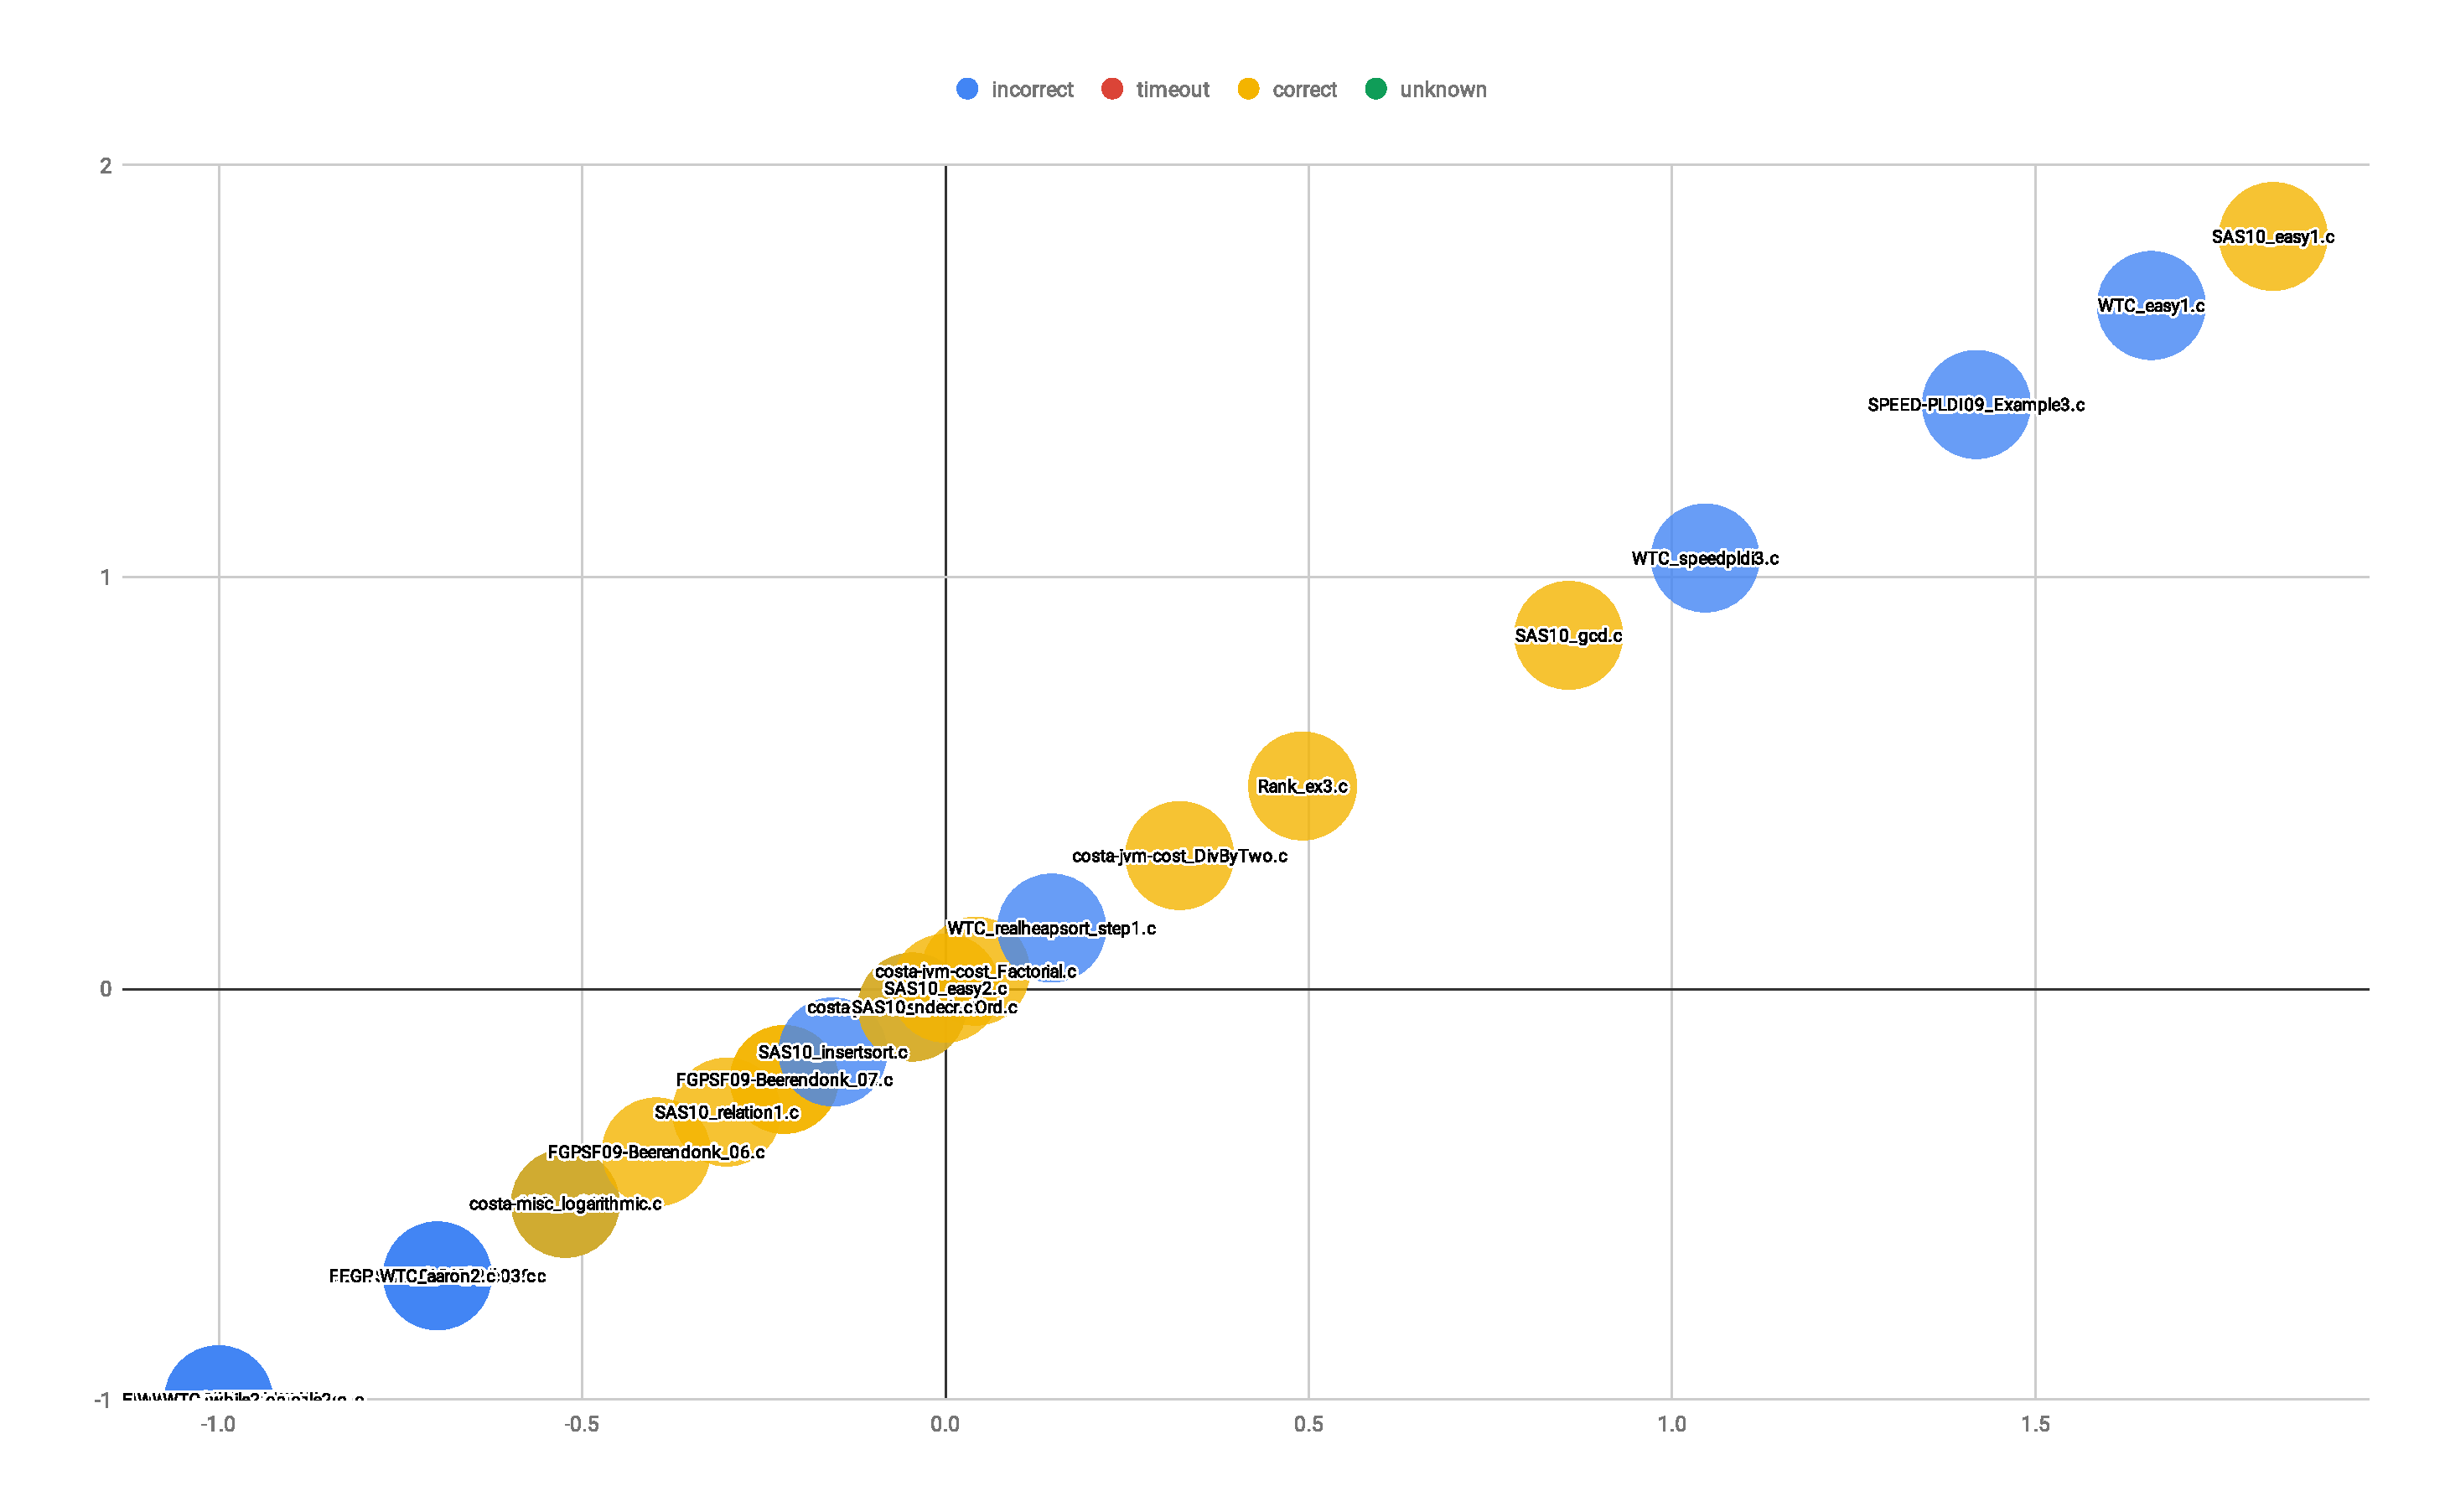
\includegraphics[width=\columnwidth]{chart.pdf}
    \caption{验证成功的测例用时(对数坐标)}
    \label{fig:chap4-performance}
\end{sidewaysfigure}

% 由于Loopus给出的上界中正确的部分较少,我们用人工的方式考察了上表中结果为错误的测例。对于其中行数较少,结构不太复杂的程序,我们对其进行复杂度分析,给出一个新的上界。我们最终得到了\todo{number}个程序的上界,比同样将它们用ACSL进行了标注。我们的工具能够顺利地验证所有这些程序的上界,说明算法对错误和正确的上界同样有效。
% !TeX root = ../main.tex

\chapter{结论}

本论文提出了程序中上界的形式化表示,以及将上界验证归约为安全属性检查问题的方法。这一自动上界验证的方法在确认算法复杂度、预测和改善程序性能以及终止性证明等方面都有一定的价值,尤其是在确证自动上界生成工具的可靠性方面很有必要。算法在\texttt{Ultimate}框架内得到了实现,并在真实程序集中进行了测试,结果显示这一方法能高效地证明或证伪大部分程序的上界。

不过本项工作的不足之处也是较为明显的。比如,从实际应用的角度来说,我们的工具由于是通过问题的归约进行验证,而安全属性检查又无法保证验证的成功,因此我们的工具也就没有相对完备性\footnote{问题本身是不可判定的,所以必然不完备。所谓相对完备(relative completeness)指的是在输入程序属于特定子类——如线性程序、确定程序等——的情况下保证求解。}。在很多验证问题中,将原问题归约为安全属性检查进行求解是比较直观的方法,但安全属性检查本身无法保证求解的问题也会随之影响上层的应用场景。究其原因,大抵在于安全属性本身表达能力较强,从而相应地判定性较弱。

因此,本论文进一步的工作方向之一便是采用其他验证方法来解决上界验证的问题。比如,在良好的约束编码情况下,基于SMT技术\cite{de_moura_satisfiability_2011}的约束求解方法可以保证较好的相对完备性,从而能拓宽工具的实际可用性;使用定理证明的方法能更准确地进行证明,但会牺牲效率等。

另一个可能的方向是放宽对程序的限制,支持更多类型的程序。比如,允许程序中存在函数调用,并在函数发生递归的情况下,通过跟踪递归的深度验证递归实例数量的上界,乃至于将函数间和函数内的验证结合起来,实现对大型实际程序和项目的支持。

上界的验证是一个一阶问题,而自动上界生成类似于程序综合(program synthesis\cite{gulwani_program_2017}),属于二阶问题,因此相对来说会更困难。我们可以和安全属性检查做一个对照:虽然它是一个一阶的验证问题,但对安全属性检查结果的验证,即对程序被证伪时给出的反例——以及与之相对应的,程序被验证为正确时所给出的证据(proof)——的验证,比安全属性检查本身要简单得多。但是对它们的验证是不可或缺的,人们逐渐认识到反例和证据的真实与否对建立工具的可靠性的意义。

验证(verification)与确证(validation)两者是相互作用的,自动上界生成也是如此。我们需要上界验证方法作为辅助,以保证工具的可靠性,甄别并杜绝计算出错误上界的情况。本论文即是在此意义上完成的。

% 其他部分
\backmatter

% 插图和附表清单
% 本科生的插图索引和表格索引需要移至正文之后、参考文献前
%\listoffiguresandtables  % 插图和附表清单
\listoffigures           % 插图清单
\listoftables            % 附表清单
\listofalgorithms

% 参考文献
\bibliography{ref/library}  % 参考文献使用 BibTeX 编译
% \printbibliography       % 参考文献使用 BibLaTeX 编译

% % !TeX root = ../main.tex

\begin{acknowledgements}
  衷心感谢我的导师王生原副教授,以及软件学院贺飞副教授对本篇论文进行的悉心指导。没有两位老师的帮助,就没有这篇论文。
  
  形式化验证是计算机科学中历久弥新的研究方向,从计算机诞生之日起,人们就在寻找增强程序可信性的方法,时至今日已经发展出了各式各样的验证技术。它涉及诸多理论,又需要对实际程序和语言的理解,因此是一个理论和实践相结合的领域。在清华大学计算机系学习的四年时间里,我逐渐感受到形式化系统以及严谨证明之美,计算机于我不再是一个单纯的机器,而是一种计算模型。感谢计算机系诸位老师的言传身教,在这里我很幸运地确立了自己的兴趣,做出了自己的选择。
  
  2019年在王生原老师处进行SRT项目时,我第一次完整地接触了形式化验证,并系统学习了形式语义学和定理证明器的有关知识;王老师教授的自动机课程,也让我感受到计算机科学完全不同的一面。虽然很遗憾后续没有再继续进行定理证明相关的研究,但在此我想特别感谢王老师将我引入这一领域,您的启蒙对我起到非常重要的作用。
  
  我还想感谢计72班的谢兴宇同学。我们都对形式化验证感兴趣,在大三的两门操作系统课上一起完成了和OS验证相关的挑战性项目。他帮助我确认了后续的研究方向,我从他那里也学习到了很多知识。此外,疫情期间我在清华大学逻辑学中心学习,和那里的老师、同学度过了非常愉快的一学期,激发了我对形式逻辑的兴趣;在中科院软件所的实习经历也让我更加深入地了解了验证领域的前沿课题,在此一并表示感谢。
  
  最后感谢一直默默陪伴我的家人和朋友们,你们总是支持着我,构成了我坚强的后盾;感谢我挚爱的恋人,你照亮了我本科最后的岁月。
\end{acknowledgements}


% 声明
% \statement[file=statement.pdf]

% 附录
\appendix

% !TeX root = ../main.tex

\begin{survey}
\label{cha:survey}

\title{
  Bound Analysis : A Brief Overview
}

\maketitle

Automatic methods for computing bounds on the resource consumption of programs are an active research field. Bound analysis, or complexity analysis, tells the potential worst-case scenario complexity of a program, and is thus useful for predicting performance. This literature review briefly documents some of the recent works on automated bound analysis. 

\tableofcontents

\section{Introduction}

Bound analysis is a branch of program analysis which attempts to determine the \textit{resource consumption} of a given program. The result is a symbolic formula over the input parameters of the program. Basically, it's the problem of deciding how many steps a Turing machine can take at most, given any input.

This is obviously an undecidable problem, since if it's decidable, we can use the decision procedure to decide the famous halting problem:

\begin{theorem}[Turing 1936\cite{turing_computable_1937}, Halting Problem]
  Given a Turing machine M and input word w, it is undecidable if M will halt on w.
\end{theorem}

Bound analysis nowadays is usually based upon \textit{termination analysis}{\cite{cook_proving_2011}}, which is the problem of deciding if a program always terminates on any input. Termination analysis is even not semi-decidable. In fact, it is neither RE nor co-RE.

The undecidability of this problem implies that, any sound method to bound analysis must be incomplete. That is, there is always an input on which the method cannot give a result. Current techniques often presume a special subset of program features that make the program class decidable (for termination), one of which is simple linear loop program. Even so, proof of a program to be terminating is not always directly appliable to bound analysis.

There are many automated bound analysis methods in the literature. We mainly focus on two methodologies in the following sections.

\section{Preliminary}

We briefly introduce some concepts here.

\begin{definition}[Transition System]
  Formally, a {\textbf{transition system}} is a pair $(S, R, I)$ where $S$ is a set of states and R is a relation of state transitions (i.e., a subset of $S \times S$). A transition from state p to state q, i.e. $(p, q) \in R$, is written as $R(p,q)$. $I$ is the set of initial states.
\end{definition}

Transition system can be seen as the most low-level model we use. On the other hand, a program has higher abstraction via CFG:

\begin{definition}[Program]
  A program is a CFG $(L, \tau, l_0)$, where L is the set of program locations, $\tau \subseteq L \times R \times L$ is the transition relation, where $R \subseteq S \times S$, and $l_0$ is a distinguished initial location.
  
  A program state is $(l, s)$ where l is a location and s is a memory state.
  
  A computation is a sequence $(l_0, s_0), (l_1, s_1), \ldots$ where for each i > 0, there is $(l_i, \rho, l_{i + 1}) \in \tau$ and $\rho (s_i, s_{i + 1})$.
  
  A program is said to be terminating if there is no infinite computation.
\end{definition}

If all the variables of a program are natural number, we can get a special case : the lossy VASS.

\begin{definition}[Lossy Vector Addition System with States]
  A VASS is a program with a fixed set of variables $\{ x_1, \ldots, x_n \}$. The edge is denoted as $x' \leqslant x + d$ with $d \in \mathbb{N}^n$.
\end{definition}

Note that variables in VASS are natural numbers, so there is a lower bound 0 for them.

\begin{definition}[Loop]
  Let G = (V, E) be a directed graph with a unique entrypoint such that all nodes are reachable from the entry point. A node a dominates a node b, if every path from entry to b includes a. An edge l1 $\rightarrow$ l2 is a back edge, if l2 dominates l1 . G is reducible, if G becomes acyclic after removing all backedges. A node is a loop header, if it is the target of a back edge. The (natural) loop of a loop header h in a reducible graph is the maximal set of nodes L such that for all x $\in$ L (1) h dominates x and (2) there is a back edge from some node n to h such that there is a path from x to node n that does not contain h.
  
  A loop-path $\pi$ is a simple cyclic path, which starts and ends at some loop header l, and visits only locations inside the natural loop of l.
\end{definition}

\begin{definition}[Inductive Invariants]
  An invariant map Q maps program locations l to state formulas $I_l$.
  
  For a program C, Q is inductive if for any $(l, l', \rho) \in \tau_C$, the following holds: 
  
  \[ \forall s, s', I_l (s) \wedge \rho (s, s') \rightarrow I_{l'} (s') \]
  
\end{definition}

\section{Control Flow Abstraction}

The tool \textit{Loopus} {\cite{sinn_simple_2014, sinn_complexity_2017, sinn_difference_2015}} utilizes an automated method of bound analysis. The algorithm is composed of 4 steps:

\begin{enumerate}
  \item Abstracting a program into a VASS
  
  \item Control Flow Abstraction, which 'flatten' the VASS and merge the loops
  
  \item Ranking function generation, which proves the VASS to be terminating
  
  \item Bound Analysis, which computes a bound for every transition.
\end{enumerate}

The first step is neglected here. The second step, \textit{control flow abstraction}, basically analysizes the program and find all the loop paths. It then transform the original VASS into a singleton state transition system with many transtion on it. The algorithm is as follows:

\begin{figure}
    \centering
    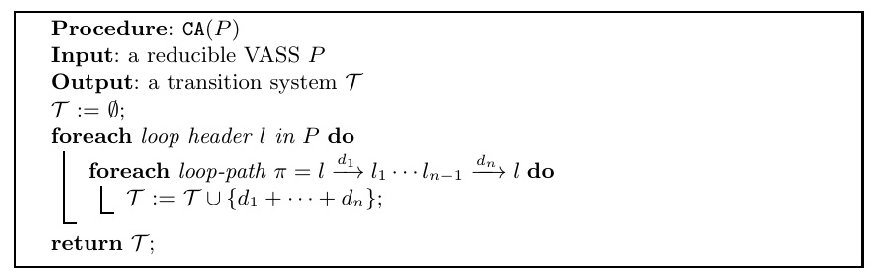
\includegraphics[width=0.8\linewidth]{survey1.pdf}
    \caption{control flow abstraction}
\end{figure}

Now we get a transition system with a single state where each transition stands for a loop path. In {\cite{sinn_simple_2014}}, the transition system is then analysized and a ranking function is generated. The ranking function is lexicographic, and each component of the ranking function is a variable among $x_1, \ldots, x_n$. In general, a ranking function could be any valid expression, thus it's possible that a single-variable ranking function does not exist. However inexpressive, this generation algorithm is relatively complete.

The last step of the analysis gives the actual bound. Suppose the transtion $\rho$ has the ranking function component x, then $\rho$ can be executed $\tmop{Init} (x)$ times if no other transitions increase x. So we have to take
other transitions into account. The algorithm is as follows:

\begin{figure}
    \centering
    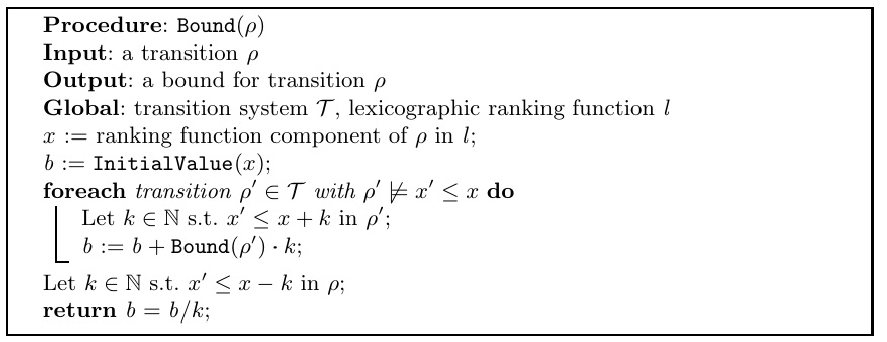
\includegraphics[width=0.8\linewidth]{survey2.pdf}
    \caption{algorithm to compute the bound}
\end{figure}

Now that a bound for each transition is obtained, we simply add them to get
the final bound.

\section{Compute WCCC using Ehrhart polynomials}

The tool \textit{Rank}{\cite{alias_multi-dimensional_2010}} gives a novel way of computing \textit{worst-case computational complexity}(WCCC). The method also generate (lexicographic) ranking function first. However, different to the method mentioned above, the ranking function can be any affine expression. Besides, since no control flow abstraction are used, the CFG is general. Thus every location in the graph is assigned a ranking function, in other words, the ranking function is inductive.

Consider any trace $(l_0, x_0), \ldots, (l_p, x_p)$, by definition of ranking function, we have $r (l_i, x_i) < r (l_{i + 1}, x_{i + 1})$, thus, every states in the trace must be distinct.

Hence the length of a trace is bounded by:

\[ \tmop{WCCC} \leqslant \# \bigcup_k r (k, P_k) \leqslant \sum_k \#r (k, P_k)
\]

The goal here is to compute $r (k, P_k)$ for each location k, where $P_k$ is the inductive invariant at location k. Basically, we find the number of points in the intersection of $\mathbb{Z}^n$ and the image of a polyhedron.

The authors use Smith normal form and Ehrhart polynomials to compute this ordinal. Suppose $r (k, x) = R x + r$, we compute $R = U S V$, where U and V are unimodular and $S = \left[ \begin{array}{cc}
  D & 0\\
  0 & 0
\end{array} \right]$ where D is diagonal positive matrix of the same rank as R. Then $\#V$ is a slight overapproximation of $\#r (k, P_k)$. The number of integer vector in V is obtained using Ehrhart polynomials.

\bibliographystyle{unsrtnat}
\bibliography{ref/library}

\end{survey}       % 本科生:外文资料的调研阅读报告
% % !TeX root = ../main.tex

\begin{translation}
\label{cha:translation}

\title{书面翻译题目}
\maketitle

\tableofcontents


本科生的外文资料书面翻译。


\section{图表示例}

\subsection{图}

附录中的图片示例(图~\ref{fig:appendix-translation-figure})。

\begin{figure}
  \centering
  \includegraphics[width=0.6\linewidth]{example-image-a.pdf}
  \caption{附录中的图片示例}
  \label{fig:appendix-translation-figure}
\end{figure}


\subsection{表格}

附录中的表格示例(表~\ref{tab:appendix-translation-table})。

\begin{table}
  \centering
  \caption{附录中的表格示例}
  \begin{tabular}{ll}
    \toprule
    文件名          & 描述                         \\
    \midrule
    thuthesis.dtx   & 模板的源文件,包括文档和注释 \\
    thuthesis.cls   & 模板文件                     \\
    thuthesis-*.bst & BibTeX 参考文献表样式文件    \\
    thuthesis-*.bbx & BibLaTeX 参考文献表样式文件  \\
    thuthesis-*.cbx & BibLaTeX 引用样式文件        \\
    \bottomrule
  \end{tabular}
  \label{tab:appendix-translation-table}
\end{table}


\section{数学公式}

附录中的数学公式示例(公式~\eqref{eq:appendix-translation-equation})。
\begin{equation}
  \frac{1}{2 \uppi \symup{i}} \int_\gamma f = \sum_{k=1}^m n(\gamma; a_k) \mathscr{R}(f; a_k)
  \label{eq:appendix-translation-equation}
\end{equation}


\section{文献引用}

文献引用示例\cite{abrahams99tex}。


% 书面翻译的参考文献
\bibliographystyle{unsrtnat}
\bibliography{ref/appendix}

% 书面翻译对应的原文索引
\begin{translation-index}
  \nocite{salomon1995advanced}
  \bibliographystyle{unsrtnat}
  \bibliography{ref/appendix}
\end{translation-index}

\end{translation}
  % 本科生:外文资料的书面翻译
%% !TeX root = ../main.tex

\begin{survey}
\label{cha:survey}
\end{survey}

% 致谢

% 生成的声明页是否要插入页眉和页脚(默认 empty)
% 仅在需要进行电子签名时,才需要打开这一选项
% 插入的扫描声明页总是会生成页眉(研究生)和页脚,不受这一选项影响
% \statement[page-style=plain]
% 将签字扫描后的声明文件 scan-statement.pdf 替换原始页面
% \statement[file=scan-statement.pdf]

% 个人简历、在学期间完成的相关学术成果
%% !TeX root = ../main.tex

\begin{resume}

  \section*{个人简历}

  1999 年 8 月 14 日出生于四川省成都市。

  2017 年 6 月考入清华大学计算机系计算机科学与技术专业攻读工学学士学位

  \section*{在学期间完成的相关学术成果}

\end{resume}


% 指导教师/指导小组学术评语
%% !TeX root = ../main.tex

\begin{comments}
% \begin{comments}[name = {指导小组学术评语}]
% \begin{comments}[name = {Comments from Thesis Supervisor}]
% \begin{comments}[name = {Comments from Thesis Supervision Committee}]

  %论文提出了……

\end{comments}


% 答辩委员会决议书
%% !TeX root = ../main.tex

\begin{resolution}

  %论文提出了……

  %论文取得的主要创新性成果包括:

  %1. ……

  %2. ……

  %3. ……

  %论文工作表明作者在×××××具有×××××知识,具有××××能力,论文××××,答辩××××。

  %答辩委员会表决,(×票/一致)同意通过论文答辩,并建议授予×××(姓名)×××(门类)学博士/硕士学位。

\end{resolution}


% 本科生的综合论文训练记录表(扫描版)
% \record{file=record.pdf}

\end{document}
